\documentclass[12pt,letterpaper,english]{amsart}
\usepackage{lmodern}
\usepackage{helvet}
\renewcommand{\familydefault}{\rmdefault}
\usepackage[T1]{fontenc}
\usepackage[latin9]{inputenc}
\usepackage{mathrsfs}
\usepackage{amsthm}
\usepackage{amstext}
\usepackage{amssymb}
\usepackage{tikz}
%\usepackage{dutchcal}
\usepackage{esint}
\usepackage{graphicx}
\usepackage{cancel}
\usepackage{comment}
%\usepackage{showkeys}
\usepackage{enumitem}
\usepackage{stmaryrd}
\usepackage{amscd,color}
\DeclareFontFamily{OT1}{pzc}{}
\DeclareFontShape{OT1}{pzc}{m}{it}{<-> s * [1.10] pzcmi7t}{}
\DeclareMathAlphabet{\mathpzc}{OT1}{pzc}{m}{it}
%\usepackage{fullpage}
%\usepackage{showkeys}
\usepackage[bbgreekl]{mathbbol}
\DeclareSymbolFontAlphabet{\mathbb}{AMSb}
\DeclareSymbolFontAlphabet{\mathbbl}{bbold}

\makeatletter

%%%%%%%%%%%%%%%%%%%%%%%%%%%%%% LyX specific LaTeX commands.
\pdfpageheight\paperheight
\pdfpagewidth\paperwidth

\newcommand{\noun}[1]{\textsc{#1}}

%%%%%%%%%%%%%%%%%%%%%%%%%%%%%% Textclass specific LaTeX commands.
\numberwithin{equation}{section}
\numberwithin{figure}{section}
\usepackage{enumitem}		% customizable list environments
\newlength{\lyxlabelwidth}      % auxiliary length 
\swapnumbers
\theoremstyle{plain}
\newtheorem{thm}[equation]{Theorem}
\theoremstyle{remark}
\newtheorem{rem}[equation]{Remark}
\theoremstyle{definition}
\newtheorem{defn}[equation]{Definition}
\theoremstyle{definition}
\newtheorem{example}[equation]{Example}
\theoremstyle{plain}
\newtheorem{cor}[equation]{Corollary}
\theoremstyle{plain}
\newtheorem{prop}[equation]{Proposition}
\theoremstyle{plain}
\newtheorem{lem}[equation]{Lemma}
\theoremstyle{plain}
\newtheorem{conj}[equation]{Conjecture} \theoremstyle{definition}
\newtheorem{notat}[equation]{Notations}
\theoremstyle{definition}
\newtheorem{exs}[equation]{Examples}

%%%%%%%%%%%%%%%%%%%%%%%%%%%%%% User specified LaTeX commands.
\usepackage{amsfonts}
\usepackage{amssymb}
\usepackage[all]{xy}
\usepackage{array}
\usepackage{lmodern}
\usepackage[T1]{fontenc}
\usepackage{bm}

\def\d{\partial}
\def\uo{\underline{0}}
\def\ul{\underline{\ell}}
\def\un{\underline{n}}
\def\uk{\underline{\kappa}}
\def\utt{\underline{\tau}}
\def\ut{\underline{t}}
\def\uv{\underline{\nu}}
\def\um{\underline{m}}
\def\uy{\underline{y}}
\def\ux{\underline{x}}
\def\uh{\underline{h}}
\def\ay{\mathbb{i}}
\def\QQ{\mathbb{Q}}
\def\RR{\mathbb{R}}
\def\CC{\mathbb{C}}
\def\UU{\mathbb{U}}
\def\FF{\mathbb{F}}
\def\ZZ{\mathbb{Z}}
\def\PP{\mathbb{P}}
\def\TT{\mathbb{T}}
\def\DD{\mathbb{D}}
\def\MM{\mathbb{M}}
\def\GG{\mathbb{G}}
\def\uz{\underline{z}}
\def\ut{\underline{t}}
\def\VV{\mathbb{V}}
\def\b{\bullet}
\def\Z{\mathcal{Z}}
\def\V{\mathcal{V}}
\def\U{\mathcal{U}}
\def\Y{\mathcal{Y}}
\def\X{\mathcal{X}}
\def\T{\mathcal{T}}
\def\Y{\mathcal{Y}}
\def\A{\mathcal{A}}
\def\B{\mathcal{B}}
\def\M{\mathcal{M}}
\def\H{\mathcal{H}}
\def\HH{\mathbb{H}}
\def\NN{\mathbb{N}}
\def\KK{\mathbb{K}}
\def\D{\mathcal{D}}
\def\vf{\varphi}
\def\vft{\tilde{\vf}}
\def\fr{\mathfrak{r}}
\def\w{\omega}
\def\ft{\mathfrak{t}}
\def\fn{\mathfrak{n}}
\def\fp{\mathfrak{p}}
\def\fg{\mathfrak{g}}
\def\sur{\twoheadrightarrow}
\def\l{\lambda}
\def\Res{\text{Res}}
\def\MHS{\mathrm{MHS}}
\def\ay{\mathbf{i}}
\def\rx{\mathrm{X}}
\def\rxc{rx^{\circ}}
\def\ve{\varepsilon}
\def\e{\epsilon}
\def\cx{\mathcal{X}}
\def\IH{\mathrm{IH}}
\def\co{\mathcal{O}}
\def\ord{\mathrm{ord}}
\def\rk{\mathrm{rk}}
\def\F{\mathcal{F}}
\def\fb{\F^{\bullet}}
\def\wb{W_{\bullet}}
\def\gr{\mathrm{Gr}}
\def\r{\mathpzc{r}}
\def\q{\mathpzc{q}}
\def\mm{\mathpzc{m}}
\def\fa{\mathfrak{a}}
\def\K{\mathcal{K}}
\def\L{\mathcal{L}}
\def\E{\mathcal{E}}
\def\KK{\mathbb{K}}
\def\EE{\mathbb{E}}
\def\C{\mathcal{C}}
\def\nf{\mathpzc{v}}
\def\v{\mathsf{v}}
\def\vt{\vartheta}
\def\fu{\mathfrak{U}}
\def\NP{\mathbbl{\Delta}}
\def\x{\mathsf{x}}
\def\y{\mathsf{y}}
\def\hx{\hat{\x}}
\def\hy{\hat{\y}}
\def\ua{\underline{a}}
\def\LL{\mathbb{L}}
\def\ui{\underline{i}}
\def\ud{\underline{d}}
\def\J{\mathcal{J}}
\def\ee{\mathbf{e}}
\def\BB{\mathbb{B}}
\def\uBB{\underline{\BB}}
\def\ub{\underline{b}}
\def\tl{\tau}
\def\qt{\mathfrak{t}}
\def\uqt{\underline{\qt}}
\def\qth{\uqt^{\hbar}}
\def\qtp{\uqt^{2\pi}}
\def\NP{\mathbbl{\Delta}}
\def\R{\mathcal{R}}
\def\RT{\tilde{\R}}
\def\uAA{\underline{\mathbb{A}}}
\def\uj{\underline{j}}
\def\uN{\underline{N}}
\def\uq{\underline{q}}
\def\fz{\mathfrak{z}}
\def\fzmn{\fz_{m,n}}
\def\fw{\mathfrak{w}}
\def\pz{\mathscr{P}_{\tilde{z}_0}^{\tilde{z}}}
\def\tz{\tilde{z}}
\def\po{\mathscr{P}_0^{\pm}}
\def\lo{\mathscr{L}_0^{\pm}}
\def\P{\mathcal{P}}
\def\mi{\text{-}}
\def\MHM{\mathrm{MHM}}
\def\sp{\mathrm{sp}}
\def\can{\mathrm{can}}
\def\van{\mathrm{van}}
\def\be{\mathbf{e}}
\def\uw{\underline{w}}
\def\sm{\setminus}
\def\ubb{\underline{\beta}}
\def\WW{\mathbb{W}}
\def\WP{\mathbb{WP}}
\def\UW{\underline{W}}
\def\UZ{\underline{Z}}
\def\ue{\underline{e}}
\def\pr{\mathrm{pr}}
\def\cs{\mathcal{S}}
\def\csb{\overline{\cs}}
\def\UX{\underline{X}}
\def\f{f'}

%\def\br#1{\sbox0{#1}\dimen0=\dimexpr\wd0+1pt\relax
%  \makebox[\dimen0]{\rlap{\vrule width\dimen0 height 0.06ex depth 0.06ex}%
 %   \rlap{\vrule width\dimen0 height\dimexpr\ht0+0.03ex\relax 
 %           depth\dimexpr-\ht0+0.09ex\relax}%
  %  \kern.5pt#1\kern.5pt}}

\def\br{\mathrm}

\newcommand{\marg}[1]{\normalsize{{\color{red}\footnote{#1}}}{\marginpar[\vskip -.3cm {\color{red}\hfill\tiny{\thefootnote}\normalsize$\implies$}]{\vskip -.3cm{ \color{red}$\impliedby$\tiny\thefootnote}}}}
\newcommand{\Matt}[1]{\marg{\color{red}(Matt): #1}}

\theoremstyle{definition}
\newtheorem*{thx}{Acknowledgments}

\makeatother

\usepackage{babel}

\renewcommand*{\thesection}{\Alph{section}}

\begin{document}

\title{Remarks on eigenspectra of isolated singularities}

\author[B. Castor]{Ben Castor}
\address{Department of Mathematics, Kenyon College, Gambier, OH}
\email{castor1@kenyon.edu}

\author[H. Deng]{Haohua Deng}
\address{Mathematics Department, Duke University, Durham, NC}
\email{haohua.deng@duke.edu}

\author[M. Kerr]{Matt Kerr}
\address{Washington University in St.~Louis, Department of Mathematics and Statistics, St.~Louis, MO}
\email{matkerr@wustl.edu}

\author[G. Pearlstein]{Gregory Pearlstein}
\address{Dipartimento di Matematica, Universit\`a di Pisa, Pisa, Italy}
\email{greg.pearlstein@unipi.it}

\subjclass[2000]{14D06, 14D07, 14J17, 32S25, 32S35}
\begin{abstract}
We introduce a simple calculus, extending a variant of the Steenbrink spectrum, for describing Hodge-theoretic invariants of (smoothings of) isolated singularities with (relative) automorphisms.  After computing these ``eigenspectra'' in the quasi-homogeneous case, we give three applications to singularity bounding and monodromy of VHS.
\end{abstract}
\maketitle

%%%%%%%%%%%%%%%%%%%%%%%%%%%%%%%
%%%%%%%%%%%%%%%%%%%%%%%%%%%%%%%
\section*{Introduction}\label{S1}

Recent work of the third author and R.~Laza on the Hodge theory of degenerations \cite{KL1,KL2} re-examined the mixed Hodge theory of the Clemens-Schmid and vanishing-cycle sequences, with an emphasis on applications to limits of period maps and compactifications of moduli.  When a degenerating family of varieties has a finite group $G$ acting on its fibers, these become exact sequences in the category of mixed Hodge structures with $G\times\mu_k$-action, where $k$ is the order of $T_{\mathrm{ss}}$ (the semisimple part of monodromy).  These kinds of situations often show up in generalized Prym or cyclic-cover constructions; for instance, instead of using the period map attached to a family of varieties, one may want to use the ``exotic'' period map arising from a cyclic cover branched along the family.
 
In this note we explain how to encode the contributions of isolated singularities with $G$-action to the vanishing cohomology in terms of \emph{$G$-spectra}.  These are formal sums (with positive integer coefficients) of triples in $\mathbb{Z} \times \mathbb{Q} \times \mathfrak{R}$, where $\mathfrak{R}$ is the set of irreducible representations of $G$. The term \emph{eigenspectrum} refers to the specific case of a cyclic group $\langle g\rangle$ with fixed generator.  In \S\ref{S1} this formalism emerges naturally from the general setting of a proper morphism of 1-parameter degenerations over a disk, by specializing the morphism to an automorphism $g\in \mathrm{Aut}(\X/\Delta)$ fixing a singularity $x\in X_0$.  The eigenspectrum $\sigma_{f,x}^g$ simply records the dimensions of simultaneous eigenspaces of $g^*$ and $T_{\mathrm{ss}}$ in the $(p,q)$-subspaces of $V_x$ (Defn.~\ref{A12}).  We give a general computation in \S\ref{S2} of $\sigma_{f,x}^g$ in the case of a quasi-homogeneous singularity, in terms of a monomial basis for the associated Jacobian ring (Cor.~\ref{B7}). 

In the remaining sections, we give three applications.  The first, in \S\ref{S3}, is to bounding the number of nodes on Calabi-Yau hypersurfaces in weighted projective spaces (Thm.~\ref{C4}) by passing to cyclic covers.  In particular, this simplifies the proof for Varchenko's bound of 135 for quintic hypersurfaces in $\PP^3$.  We also obtain the curious result that a CY hypersurface in $\PP^{n+1}$ with isolated singularities and symmetric under $\mathfrak{S}_{n+2}$ cannot contain a node whose $\mathfrak{S}_{n+2}$-orbit has cardinality $(n+2)!$ (Thm.~\ref{C9}).

The other two applications concern codimension-one monodromy phenomena for VHSs over moduli of configurations of points and hyperplanes.  In \S\ref{S4}, the moduli space is $M_{0,2n}$, with the VHS arising from cyclic covers of $\PP^1$ branched along the $2m$ ordered points.  Propositions \ref{D5}-\ref{D6} describe the eigenspectra for boundary strata of certain compactifications $\overline{M}^H_{0,2n}$ due to Hassett \cite{Ha}, also closely related to work of Deligne and Mostow \cite{DM}; this generalizes a computation of \cite{GKS}.  

Our other main example, treated in \S\ref{S5}, is the VHS $\mathcal{H}\to\mathcal{S}$ on the moduli space of general configurations of $(2n+2)$ hyperplanes in $\PP^n$, arising from the middle (intersection) cohomology of a 2:1 cover $X\to \PP^n$ branched along these hyperplanes.  By passing to a smooth complete intersection $2^{2n}$-cover of $X$ and applying the Cayley trick, we replace $X$ by a smooth hypersurface $Y\subset \PP(\co_{\PP^{2n+1}}(2)^{\oplus (n+1)})$ with automorphisms by a group of order $2^{2n}$.  In codimension-one in moduli, $Y$ acquires nodes, and a variant of Schoen's result in \cite{Sc} ensures that these produce nontrivial symplectic transvections for $\H$ when $n$ is odd.  This gives an easy proof that the geometric monodromy group of $\H$ is maximal (for all $n$), and the period map ``non-classical'', a fact first proved by \cite{GSVZ} for $n=3$ and by \cite{SXZ} in general.

\subsection*{Notation}
In this paper ``MHS'' stands for $\QQ$-mixed Hodge structure.  We shall make frequent use of the \emph{Deligne bigrading} on a MHS $V$ \cite{De2}.  This is (by definition) the unique decomposition $V_{\CC}=\oplus_{p,q\in \ZZ} V^{p,q}$ with the properties that $F^k V_{\CC}=\oplus_{\substack{p,q \\ p\geq k}}V^{p,q}$, $W_{\ell}V_{\CC}=\oplus_{\substack{p,q \\ p+q\leq \ell}}V^{p,q}$, and $\overline{V^{q,p}}\equiv V^{p,q}$ mod $\oplus_{\substack{a<p \\ b<q}}V^{a,b}$.  We shall make free use of standard multi-index notation (for $n$-tuples of variables or field-elements) to simplify formulas, viz. $\uz=(z_1,\ldots,z_n)$, $\CC[\uz]=\CC[z_1,\ldots,z_n]$, $\uz^{\um}=\prod_i z_i^{m_i}$, $\um\cdot \uw=\sum_i m_iw_i$, $|\um|=\sum_i m_i$, $\ue^{(i)}=$  $i^{\text{th}}$ standard basis vector, etc.

\begin{thx}
We thank P.~Gallardo and R.~Laza for valuable discussions related to this paper.  This work was partially supported by Simons Collaboration Grant 634268 and NSF Grant DMS-2101482 (MK).  MK and GP would also like to thank the Isaac Newton Institute for Mathematical Sciences for support and hospitality during the programme ``$K$-theory, algebraic cycles, and motivic homotopy theory'' (supported by EPSRC Grant Number EP/R014604/1) when work on this paper was undertaken.
\end{thx}

%%%%%%%%%%%%%%%%%%%%%%%%%%%%%%%%%%%%%%
%%%%%%%%%%%%%%%%%%%%%%%%%%%%%%%%%%%%%%
\section{$G$-spectra and eigenspectra}\label{S1}

We begin in the general setting of a proper morphism
\begin{equation}\label{A1}
\xymatrix{\Y \ar [rr]^{\pi} \ar [rd]_{\f} && \X \ar [ld]^f \\ & \Delta }
\end{equation}
of complex analytic spaces over a disk, which we assume is the restriction to $\Delta$ of a proper morphism of quasi-projective varieties over an algebraic curve.  (In particular, at the level of fibers we have that $\pi_t\colon Y_t\to X_t$ is a proper algebraic morphism of quasi-projective varieties.) Let $\K^{\b}\in D^b\mathrm{MHM}(\X)$ and $\L^{\b}\in D^b\mathrm{MHM}(\Y)$ be given, with a morphism $\rho\colon \K^{\b}\to R\pi_*\L^{\b}$.  Writing $\imath\colon X_0\hookrightarrow \X$ for the inclusion, the vanishing cycle triangle
\begin{equation}\label{A2}
\imath^*\overset{\mathrm{sp}}{\longrightarrow}\psi_f \overset{\mathrm{can}}{\longrightarrow}\phi_f \overset{\delta}{\underset{[+1]}{\longrightarrow}}
\end{equation}
consists of functors from $D^b\mathrm{MHM}(\X)$ to $D^b\mathrm{MHM}(X_0)$, with natural transformations between them; moreover, monodromy $T=T_{\mathrm{ss}}e^N$ induces natural automorphisms of $\psi_f$ and $\phi_f$.  By proper base-change and faithfulness of $\mathrm{rat}\colon D^b\mathrm{MHM}(X_0)\to D^b_c(X_0)$, $R\pi_*\colon D^b\MHM(Y_0)\to D^b \MHM(X_0)$ intertwines the corresponding triangle (and monodromy actions) for $(\Y,\f)$.  Taking hypercohomology on $X_0$ yields:

\begin{prop}\label{A3}
We have the commutative diagram\small
\[\xymatrix@C=13pt{\to \HH^k(X_0,\imath^*\K^{\b}) \ar [r]^{\sp}	\ar [d]^{\rho} & \HH^k(X_0,\psi_f\K^{\b}) \ar [r]^{\can} \ar [d]^{\rho} & \HH^k(X_0,\phi_f\K^{\b}) \ar [r]^{\delta\mspace{25mu}} \ar [d]^{\rho} & \HH^{k+1}(X_0,\imath^*\K^{\b})\to \ar [d]^{\rho}\\ \to \HH^k(Y_0,\imath^*\L^{\b}) \ar [r]^{\sp} & \HH^k(Y_0,\psi_{\f}\L^{\b}) \ar [r]^{\can} & \HH^k(Y_0,\phi_{\f}\L^{\b}) \ar [r]^{\delta\mspace{25mu}} & \HH^{k+1}(Y_0,\imath^*\L^{\b})\to }
\]\normalsize
with rows the vanishing-cycle \textup{(}long-exact\textup{)} sequences, in which all arrows are morphisms of MHS. Moreover, the diagram intertwines the actions of $T_{\mathrm{ss}}$ \textup{(}by automorphisms of MHS\textup{)} and $N$ \textup{(}by nilpotent $(-1,-1)$-endomorphisms of MHS\textup{)}, which are trivial \textup{(}$\mathrm{Id}$ resp.~$0$\textup{)} on the end terms.
\end{prop}

\begin{rem}\label{A4}
If $f,\f$ are themselves projective (hence proper), and $\K^{\b},\L^{\b}$ semisimple with respect to the perverse $t$-structure (e.g.~$\K^{\b}=\mathcal{IC}_{\X}^{\b}$, $\L^{\b}=\mathcal{IC}_{\Y}^{\b}$), then the Decomposition Theorem applies, yielding Clemens-Schmid sequences (cf.~\cite[\S5]{KL1}) which are then automatically compatible under $\rho$. The main consequence is that the local invariant cycle theorem holds, i.e.~$\sp$ surjects onto the $T$-invariants.
\end{rem}

Next, assume $\X,\Y,\{X_t\}_{t\neq 0}$, and $\{Y_t\}_{t\neq 0}$ are smooth, and take $\L^{\b}=\QQ_{\Y}$ and $\K^{\b}=\QQ_{\X}$; then the diagram in Prop.~\ref{A3} becomes 
\begin{equation}\label{A5}
\xymatrix{\to H^k(X_0) \ar [r]^{\sp} \ar [d]^{\pi^*} & H^k_{\lim}(X_t) \ar [r]^{\can} \ar [d]^{\pi^*} & H^k_{\van}(X_t) \ar [r]^{\delta\mspace{25mu}} \ar [d]^{\pi^*} & H^{k+1}(X_0) \to \ar [d]^{\pi^*} \\ \to H^k(Y_0) \ar [r]^{\sp}  & H^k_{\lim}(Y_t) \ar [r]^{\can}  & H^k_{\van}(Y_t) \ar [r]^{\delta\mspace{25mu}}  & H^{k+1}(Y_0) \to .}
\end{equation}
Now if $n=\dim X_0$ and $\Sigma:=\mathrm{sing}(X_0)$ is finite, then $H^k_{van}(X_t)=\{0\}$ for $k\neq n$ and, defining $V_x:=H^0\imath_x^*\phi_f\QQ_{\X}[n]$, 
\begin{equation}\label{A6}
H^n_{\van}(X_t)\cong \textstyle \bigoplus_{x\in \Sigma} V_x
\end{equation}
as MHS.  We have of course $\pi^{-1}(\Sigma)\subset \widetilde{\Sigma}:=\mathrm{sing}(Y_0)$, and if $\dim Y_0 = n$ and $|\widetilde{\Sigma}|<\infty$ then, writing $\widetilde{V}_y:=H^0\imath_y^*\phi_{\f}\QQ_{\Y}[n]$ ($y\in \widetilde{\Sigma}$), $\pi^*$ restricts to morphisms
\begin{equation}\label{A7}
[\pi^*]_x\colon V_x\to \textstyle\bigoplus_{y\in \pi^{-1}(x)}\widetilde{V}_y 
\end{equation}
of $T$-MHS --- i.e.~morphisms of MHS intertwining $T$ (hence $T_{\mathrm{ss}}$ and $N$).  These are local invariants.

Recall that $T_{\mathrm{ss}}$ acts through finite cyclic groups on each $V_x$ (and $\widetilde{V}_y$), and let $\kappa$ be the $lcm$ of their orders.  Write $\zeta_{\kappa}:=e^{\frac{2\pi\ay}{\kappa}}$ and $V_{x,\be(\frac{a}{\kappa})}^{p,q}$ for the $\be(\tfrac{a}{\kappa}):=e^{2\pi\ay\frac{a}{\kappa}}=\zeta_{\kappa}^a$-eigenspace of $T_{\mathrm{ss}}$ in $V_x^{p,q}\subset V_{x,\CC}$.  The explicit choice of $\zeta_{\kappa}\in \CC$ is needed to make the following

\begin{defn}\label{A8}
The \emph{mixed spectrum} $\sigma_{f,x}$ of the isolated singularity $x\in \Sigma$ is the element $\sum_{\alpha,w}m_{\alpha,w}^{f,x}(\alpha,w)$ of the free abelian group $\ZZ\langle \QQ\times \ZZ\rangle$, where $m_{\alpha,w}^{f,x}=\dim(V_{x,\be(\alpha)}^{\lfloor\alpha\rfloor,w-\lfloor\alpha\rfloor})$.\footnote{Here $\lfloor\cdot\rfloor$ is the greatest integer (floor) function; note also that $\be(\alpha)$ is equivalent to taking the fractional part $\{\alpha\}:=\alpha-\lfloor\alpha\rfloor$ of $\alpha$	.}
\end{defn}
\noindent Evidently \eqref{A7} must be compatible with the decompositions recorded by the mixed spectra.

Now let $\mathcal{G}\leq \mathrm{Aut}(\X/\Delta)$, with $\X$ and $\{X_t\}_{t\neq 0}$ smooth and $|\Sigma|<\infty$.  Applying the foregoing results with $\Y=\X$, $f=f'$, and $\pi:=g\in \mathcal{G}$, together with \cite[Prop.~5.5(i)]{KL1}, yields

\begin{cor}\label{A9}
The vanishing-cycle sequence
\begin{equation}\label{A10}
0\to H^n(X_0)	\overset{\sp}{\to}H^n_{\lim}(X_t)\overset{\can}{\to}\textstyle\bigoplus_{x\in \Sigma}V_x \overset{\delta}{\to}H^{n+1}_{\mathrm{ph}}(X_0)\to 0
\end{equation}
is an exact sequence of $\mathcal{G}\times\mu_{\kappa}$-MHS,\footnote{Again, this means that the action of $\mathcal{G}$ and $T_{\text{ss}}$ on the MHSs (as automorphisms of MHS) commute with each other and with $\sp$, $\can$, and $\delta$.} where the $\langle T_{\text{ss}}\rangle\cong \mu_{\kappa}$-action on the end terms is trivial.  If $\X/\Delta$ is proper, then $H^{n+1}_{\mathrm{ph}}(X_0):=\ker(\sp)\subseteq H^{n+1}(X_0)$ is pure of weight $n+1$.
\end{cor}

The decomposition of terms in \eqref{A10} into irreps for $\mathcal{G}\times\mu_{\kappa}$ only becomes useful if we understand the action on the vanishing cohomology $\bigoplus_{x\in\Sigma}V_x$ for a given collection of singularities.  In particular, if $gx=x$ then we need to further refine the spectrum under the resulting automorphism $g^*\colon V_x\to V_x$ of $T$-MHS.

\begin{defn}\label{A11}
Write $G\leq \mathrm{stab}(x)\leq \mathcal{G}$, and $\mathcal{R}_G$ for the set of complex irreducible representations of $G$.  The \emph{$G$-spectrum} $\sigma_{f,x}^G$ of $x$ is the element $\sum_{(\alpha,w,U)}m^{f,x,G}_{\alpha,w,U}(\alpha,w,U)$ of the free abelian group $\ZZ\langle\QQ\times \ZZ\times \mathcal{R}_G\rangle$, where (for each $(\alpha,w)$) $V_{x,\be(\alpha)}^{\lfloor\alpha\rfloor,w-\lfloor\alpha,\rfloor}\cong \bigoplus_{U\in \mathcal{R}_G}U^{\oplus m^{f,x,G}_{\alpha,w,U}}$ as $G$-representations.
\end{defn}

In the special case where $G=\langle g\rangle\cong \mu_{\ell}$ is cyclic, the $\CC$-irreps are characters indexed by the power $\zeta_{\ell}^c=e^{2\pi\ay\frac{c}{\ell}}$ of $\zeta_{\ell}$ to which $g$ is sent.

\begin{defn}\label{A12}
The \emph{eigenspectrum} of an isolated singularity $x$ with automorphism $g$ is the element $$\sigma^g_{f,x}=\sum_{(\alpha,w,\gamma)}m^{f,x,g}_{\alpha,w,\gamma}(\alpha,w,\gamma)\in \ZZ\langle \QQ\times\ZZ\times\QQ/\ZZ\rangle,$$ where $m^{f,x,g}_{\alpha,w,\gamma}$ is the dimension of the eigenspace $(V^{\lfloor\alpha\rfloor,w-\lfloor\alpha,\rfloor}_{x,\be(\alpha)})^{\be(\gamma)}\subseteq V_{x,\be(\alpha)}^{\lfloor\alpha\rfloor,w-\lfloor\alpha\rfloor}$ for $g^*$ with eigenvalue $\be(\gamma)=e^{2\pi\ay\gamma}$.
\end{defn}

\begin{rem}\label{A13}
For $\X/\Delta$ proper (with hypotheses as in Cor.~\ref{A9}), $H^n(X_t)$ is a VHS on $\Delta^*$ whose automorphism group contains $\mathcal{G}$. For any field extension $K/\QQ$, this decomposes as $K$-VHS into a direct sum of $\mathcal{G}$-isotypical components, corresponding to $K$-irreps of $\mathcal{G}$.  The $\mathcal{G}$-action on and decomposition of $H^n_{\lim}(X_t)$ obtained by taking limits are the same as those arising from the $\mathcal{G}$-MHS structure on $H^n_{\lim}(X_t)$ in Cor.~\ref{A9}.
\end{rem}

We now turn to the explicit computation of these eigenspectra in the simplest case.



%%%%%%%%%%%%%%%%%%%%%%%%%%%%%%%
%%%%%%%%%%%%%%%%%%%%%%%%%%%%%%%
\section{Quasihomogeneous singularities with automorphism}\label{S2}

Let $F\in \CC[z_1,\ldots,z_{n+1}]$ (with $n>0$) be a \emph{quasi-homogeneous polynomial} with an isolated singularity at the origin $\uo$.  That is, choosing a weight vector $\uw=(w_1,\ldots,w_{n+1})\in \QQ_{>0}^{n+1}$ and setting $$\mathfrak{M}_{\uw}:=\{\um\in \ZZ_{\geq 0}^{n+1}\mid \um\cdot \uw=1\},$$ we have 
\begin{equation}\label{B1}
F=\sum_{\um\in \mathfrak{M}_{\uw}}a_{\um}\uz^{\um}
\end{equation}
for some $a_{\um}\in \CC$.  We recall that the \emph{degree} $\kappa_F$ of $F$ is the least integer such that $\kappa_F w_i\in \NN$ for $i=1,\ldots,n+1$; define $w_i:=\kappa_F w_i$ and set $\uk:=(\kappa_1,\ldots,\kappa_{n+1})$.

Next recall the setting of Defn.~\ref{A8}, where $f\colon \X\to \Delta$ is a holomorphic map with quasi-projective fibers and smooth total space, with $X_t$ smooth for $t\neq 0$ and $\mathrm{sing}(X_0)=:\Sigma$ finite.  A singularity $x\in \Sigma\subset X_0$ is \emph{quasi-homogeneous} if $f$ can be locally analytically identified with \eqref{B1} for some $\uw$.  In that case, $V_x$ and $\sigma_{f,x}$ identify with the vanishing cohomology
\begin{equation}\label{B2}
V_F:=H^0\imath^*_{\uo}\phi_F \QQ_{\CC^{n+1}}
\end{equation}
of $F\colon \CC^{n+1}\to \CC$ at $\uo$, and its mixed spectrum $\sigma_F$.  These were first computed by Steenbrink in \cite{St}, and we briefly review the treatment from \cite[\S2]{KL2} before passing to eigenspectra.

Writing $J_F:=(\tfrac{\d F}{\d z_1},\ldots ,\tfrac{\d F}{\d z_{n+1}})\subseteq \CC[\uz]$ for the Jacobian ideal, let $\mathcal{B}\subset \ZZ_{\geq 0}^{n+1}$ be chosen so that the monomials $\{\uz^{\underline{\beta}}\}_{\underline{\beta}\in \mathcal{B}}$ provide a basis of $\CC[\uz]/J_F$.  Write $\mu_F:=|\mathcal{B}|$ for the \emph{Milnor number} of $F$, and $\ell(\underline{\beta}):=\tfrac{1}{\kappa_{F}}\sum_{i=1}^{n+1}\kappa_i(\beta_i+1)=\sum_{i=1}^{n+1}w_i(\beta_i+1)$.

\begin{prop}\label{B3}
We have $\mu_F=\dim V_F$ for the Milnor number and
$$\sigma_F=\textstyle\sum_{\underline{\beta}\in \mathcal{B}}(\alpha(\underline{\beta}),w(\underline{\beta}))\in \ZZ\langle \QQ\times \ZZ\rangle$$
for the mixed spectrum, where $\alpha(\underline{\beta}):=n+1-\ell(\underline{\beta})$ and $w(\underline{\beta}):=n$ \textup{[}resp. $n+1$\textup{]} if $\alpha(\underline{\beta})\notin \ZZ$ \textup{[}resp. $\in \ZZ$\textup{]}.
\end{prop}

\begin{proof}[Sketch]
Perform a base-change followed by weighted blow-up at $\uo$
\begin{equation}\label{B4}
\xymatrix@R=0.8pc{\CC^{n+1} \ar [d]_F & \mathfrak{X} \ar [d]_{\hat{F}} \ar [l] & \mathfrak{Y} \ar [l]_{\mathrm{Bl}_{\underline{\kappa}}} \ar [ld]^{\widetilde{F}}	\\
\CC & \Delta \ar [l] \\ t^{\kappa_F} & t \ar @{|->} [l]}
\end{equation}
with exceptional divisor $\E=\{T^{\kappa_F}=F(\underline{Z})\}\subset \mathbb{WP}[1{:}\underline{\kappa}]=:\mathbf{P}$ (in weighted homogeneous coordinates $T,Z_1,\ldots,Z_{n+1}$).  The singular fiber $\mathbb{Y}_0:=\widetilde{F}^{-1}(0)$ is the union of $\E$ and the proper transform $\widetilde{\mathbb{X}}_0$ of $\mathbb{X}_0:=F^{-1}(0)=\hat{F}^{-1}(0)$, meeting in 
$$E:=\E\cap \widetilde{\mathbb{X}}_0=\{F(\underline{Z})=0\}\subset \mathbf{H}:=\{T=0\}\,(\cong \mathbb{WP}[\underline{\kappa}])\subset \mathbf{P}.$$

The claim is then that $V_F\cong H^n(\E\setminus E)$, which can be checked using \eqref{A5} with $\pi=\mathrm{Bl}_{\underline{\kappa}}$.  Since $E$ [resp. $\uo$] is a deformation retract of $\mathbb{Y}_0$ [resp. $\mathbb{X}_0$], while $\mathbb{Y}_t=\mathbb{X}_t$ for $t\neq 0$, and $\phi_{\widetilde{F}}\QQ_{\mathcal{Y}}\simeq \imath^E_*\QQ_E(-1)[-1]$ (cf.~\cite[6.3 and 8.3-4]{KL1}), the diagram becomes
$$\xymatrix@C=1pc{&0\ar[r] & H^n_{\lim}(\mathbb{X}_t)\ar [r]^{\cong} \ar @{=} [d] & V_F \ar [d]^{\mathrm{Bl}^*} \ar [r] & 0 \\ H^{n-2}(E)(-1)\ar [r] & H^n(\E) \ar [r] & H^n_{\lim}(\mathbb{Y}_t) \ar [r] & H^{n-1}(E)(-1) \ar [r] & H^{n+1}(\E)}$$
whence the result.

Next, one constructs a basis of $H^n(\E\sm E)$ from $\mathcal{B}$, using residue theory.  Writing (with $T:=Z_0$) 
$$\Omega_{\mathbf{P}}=\sum_{j=0}^{n+1} (-1)^j Z_j\, dZ_0\wedge\cdots \wedge \widehat{dZ_j}\wedge \cdots \wedge dZ_{n+1},$$
for each $\underline{\beta}\in \mathcal{B}$ we set (with $\underline{Z}^{\underline{\beta}}=Z_1^{\beta_1}\cdots Z_{n+1}^{\beta_{n+1}}$)
\begin{equation}\label{B5}
\Omega_{\underline{\beta}}:=\frac{T^{\kappa_F}\underline{Z}^{\underline{\beta}}\Omega_{\mathbf{P}}}{T(F(\underline{Z})-T^{\kappa_F})^{\lceil \ell(\underline{\beta})\rceil}}\in \Omega^{n+1}(\mathbf{P}\sm\E\cap\mathbf{H})
\end{equation}
and $\omega_{\underline{\beta}}:=\mathrm{Res}_{\E\sm E}([\Omega_{\underline{\beta}}])\in H^n(\E\sm E)$.  We refer to \cite[Thm.~2.2]{KL2} for the proof that this has $(p,q)$-type $(\lfloor\alpha(\underline{\beta})\rfloor,\lfloor\ell(\underline{\beta})\rfloor)$, and \cite[Thm.~1]{St} for the assertion that the $\{\omega_{\underline{\beta}}\}$ give a basis.  Note that $\lfloor\alpha(\underline{\beta})\rfloor+\lfloor\ell(\underline{\beta})\rfloor=w(\underline{\beta})$.

Finally, the action of $T_{\text{ss}}$ is computed by $T\mapsto \zeta_{\kappa_F}T$, or equivalently (in weighted projective coordinates) by $Z_i\mapsto \zeta_{\kappa_F}^{-\kappa_i}Z_i=e^{-2\pi\ay w_i}Z_i$.  Clearly the effect of this on \eqref{B5} is to multiply it by $e^{2\pi\ay\sum w_i(\beta_i+1)}=e^{2\pi\ay\alpha(\underline{\beta})}$, as desired.
\end{proof}

Now given a finite group $G\leq \mathrm{Aut}(\X/\Delta)$ fixing $x\in \Sigma$, we can always choose local holomorphic coordinates on which the action is linear \cite{Ca}.  So for a given $g\in G$, we can choose coordinates to make the action diagonal, through roots of unity. Accordingly, we shall compute the eigenspectrum in the case where $g\in \mathrm{Aut}(\CC^{n+1},\uo)$ is given by
\begin{equation}\label{B6}
g(z_1,\ldots,z_{n+1}):=(\zeta_{\ell}^{c_1}z_1,\ldots,\zeta_{\ell}^{c_{n+1}}z_{n+1})	
\end{equation}
and $F\in \CC[\uz]^{\langle g\rangle}$ is a $g$-invariant quasi-homogeneous polynomial.  In fact, taking $\mathcal{B}\subset \ZZ^{n+1}_{\geq 0}$ as above, we have the

\begin{cor}\label{B7}
The eigenspectrum $\sigma_F^g$ is given by
$$\sum_{\underline{\beta}\in \mathcal{B}}(\alpha(\underline{\beta}),w(\underline{\beta}),\gamma(\underline{\beta}))\in \ZZ\langle \QQ\times\ZZ\times\QQ/\ZZ\rangle,$$	
where $\gamma(\underline{\beta}):=\frac{1}{\ell}\sum_{i=1}^{n+1}c_i(\beta_i+1)$.
\end{cor}
\begin{proof}
We only need to compute the action of $g^*$ on $\omega_{\underline{\beta}}$, which is to say the effect of $Z_i\mapsto \zeta_{\ell}^{c_i}Z_i$ on $\underline{Z}^{\underline{\beta}}\Omega_{\underline{\beta}}$.  Clearly this is just multiplication by $\zeta_{\ell}^{\sum c_i(\beta_i+1)}=e^{2\pi\ay\gamma(\underline{\beta})}$.	
\end{proof}

\begin{example}\label{B8}
For a Brieskorn-Pham singularity $F=\sum_{i=1}^{n+1}z_i^{\lambda_i}$ ($\lambda_i=\tfrac{1}{w_i}=\tfrac{\kappa_F}{\kappa_i}$), we have $\mathcal{B}=\times_{i=1}^{n+1}\{\ZZ\cap[0,d_i-2]\}$.  Hence, writing $\Gamma_m=\sum_{j=1}^{m-1}[\tfrac{j}{m}]$ in the group ring $\ZZ[\QQ]$ (with product $*$), we have $\sum_{\underline{\beta}\in \mathcal{B}}[\alpha(\underline{\beta})]=\Gamma_{\lambda_1}*\cdots*\Gamma_{\lambda_{n+1}}$. This extends to $\sum_{\underline{\beta}\in \mathcal{B}}[(\alpha(\ubb),\gamma(\ubb))]=\widetilde{\Gamma}_{\lambda_1}(\tfrac{c_1}{\ell})*\cdots*\widetilde{\Gamma}_{\lambda_{n+1}}(\tfrac{c_{n+1}}{\ell})$ in the group ring $\ZZ[\QQ\times(\QQ/\ZZ)]$ if we write $\widetilde{\Gamma}_m(\tfrac{c}{\ell})=\sum_{j=1}^{m-1}[(\tfrac{m-j}{m},\tfrac{jc}{\ell})]$.	
\end{example}

\begin{rem}\label{B9}
The eigenspectrum of a $\mu$-constant (semi-quasi-\linebreak homogeneous) deformation of $(F,\gamma)$ remains constant.  Even in the more general case of \cite[\S5.2]{KL2}, one can in principle still use the action of $\gamma^*$ on the (local) Jacobian ring $\co_{n+1}/J_F$ to refine $\sigma_F$ to $\sigma_F^g$. But Corollary \ref{B7} (and quasi-homogeneous deformations of Example \ref{B8}) will suffice for our purposes below.
\end{rem}




%%%%%%%%%%%%%%%%%%%%%%%%%%%%%%%


%%%%%%%%%%%%%%%%%%%%%%%%%%%%%%%
%%%%%%%%%%%%%%%%%%%%%%%%%%%%%%%
\section{Bounding nodes on Calabi-Yau hypersurfaces}\label{S3}


Let $\WW=\WP[e_0:\cdots:e_{n+1}]$ be a weighted projective $(n+1)$-space with finitely many singularities.\footnote{We may assume (without loss of generality) that no $n+1$ of the $e_i$ have a common factor.} Suppose we want to bound (numbers and types of) singularities on a hypersurface $X_0=\{F_0(\UW)=0\}\subset \WW$ of degree $d$, where a smooth such hypersurface would have Hodge numbers $\uh=(h^{n,0},h^{n-1,1},\ldots ,h^{0,n})$.  Write $d_i=\tfrac{d}{e_i}$ for $i=0,\ldots,n+1$.

We shall assume that the singularities of $X_0$ are all isolated. Taking a general deformation $F_t=F_0+tG$ to produce a family of $f\colon \X\to \Delta$ with smooth total space, the vanishing-cycle sequence
\begin{equation}\label{C1}
0\to H^n(X_0)\to H^n_{\lim}(X_t)\to \textstyle\bigoplus_{x\in \Sigma}V_x \overset{\delta}{\to} H^{n+1}_{\text{ph}}(X_0)\to 0
\end{equation}
offers a naive such bound: first, by Schmid's nilpotent orbit theorem, the rank of $\gr_F^p$ remains constant in the limit, giving the second equality of 
\begin{equation}\label{C2}
h^{p,n-p}=h^{p,n-p}(X_t)=\textstyle\sum_q h^{p,q}_{\lim}(X_t)\geq \sum_q h^{p,q}(\ker(\delta)).	
\end{equation}
Moreover, the mixed spectrum $\sigma_{f,x}$ tells us the $h^{p,q}_{\zeta}(V_x)=\dim(V^{p,q}_{x,\zeta})$ (for each eigenvalue $\zeta$ of $T_{\text{ss}}$), and only the $V_{x,1}^{p,n+1-p}$ can map nontrivially under $\delta$.  Since the hyperplane class also has $T_{\text{ss}}$-eigenvalue $1$, \eqref{C2} forces $\sum_q\sum_{\zeta\neq 1}\dim(V^{p,q}_{x,\zeta})\leq h^{p,n-p}_{\text{pr}}$.

When $x$ is a node, i.e. $f\overset{\text{loc}}{\sim}\sum_{i=1}^{n+1}z_i^2$, Prop.~\ref{B3} gives $V_{x,\CC}=V^{\frac{n}{2},\frac{n}{2}}_{x,-1}$ for $n$ even and $V_{x,1}^{\frac{n+1}{2},\frac{n+1}{2}}$ for $n$ odd.  In the latter case, \eqref{C2} yields no immediate bound on the number of nodes (though one does have results like \cite[Thm.~2.9+Cor~2.11]{KL2}).  For $n=2m$ even, \eqref{C2} yields\footnote{This is by the same residue theory as used in the proof of Theorem \ref{C4} below. The notation `$*$' is from Example \ref{B8}.}
\begin{equation}\label{C3}
h^{\frac{n}{2},\frac{n}{2}}_{\text{pr}}(X_t)=\,\text{coefficient of $[\tfrac{n}{2}+1]$ in $\Gamma_{d_0}*\Gamma_{d_1}*\cdots *\Gamma_{d_{n+1}}$}
\end{equation}
as a bound, which while better than nothing is rather weak.

\begin{example}\label{CE}
The simplest nontrivial case is $\WW=\PP^3$ ($n=2$) and ($d_0=d_1=d_2=d_3=$)$\,d=4$, where $\Gamma_4^{*4}=([\tfrac{1}{4}]+[\tfrac{1}{2}]+[\tfrac{3}{4}])^{*4}=$
\begin{equation}\label{Ce}
[1]+4[\tfrac{5}{4}]+10[\tfrac{3}{2}]+16[\tfrac{7}{4}]+19[2]+16[\tfrac{9}{4}]+10[\tfrac{5}{2}]+4[\tfrac{11}{4}]+[3]
\end{equation}
correctly gives $19=h^{1,1}_{\text{pr}}(X_t)$.  This is also a poor bound for the number of nodes on a quartic surface (cf. Example \ref{C6}).
\end{example}

However, there is a simple trick which improves the bound while also giving one for odd $n$:

\begin{thm}\label{C4}
The number of nodes on $X_0$ is bounded by the coefficient, in $\Gamma_{d_0}*\Gamma_{d_1}*\cdots*\Gamma_{d_{n+1}}$, of $[\tfrac{n+1}{2}+\tfrac{1}{2d}]$ if $n$ is even and $d$ is odd, or of $[\tfrac{n+1}{2}+\tfrac{1}{d}]$ otherwise.	
\end{thm}
\begin{proof}
Let $Y_t=\{F_t(\UW)+W_{n+2}^d=0\}\subset \WP[\ue{:}1]=:\widetilde{\WW}$ be the cyclic $d{:}1$-cover of $\WW$ branched over $X_t$, with $g\colon W_{n+2}\mapsto \zeta_d W_{n+2}$ the cyclic automorphism. By Dolgachev's extension of Griffiths's residue theory \cite{Do}, a basis for the $g^*$-eigenspace $H^{n-q+1,q}_{\text{pr}}(Y_t)^{\bar{\zeta}_d^j}$ ($t\neq 0$, $0\leq j<d$) is given by the Poincar\'e residue classes $$\mathrm{Res}_{Y_t}\left(\frac{\UW^{\underline{k}-\underline{1}}W_{n+2}^{d-j-1}\Omega_{\widetilde{\WW}}}{(F_t+W_{n+2}^d)^{q+1}}\right)$$
with $k_i\in \ZZ\cap (0,d_i)$ ($i=0,\ldots,n+1$) and weights of numerator and denominator equal:  that is, $\sum_{i=0}^{n+1}e_ik_i+(d-j)=(q+1)d$, or equivalently (dividing by $d$) $\sum_{i=0}^{n+1}\tfrac{k_i}{d_i}=q+\tfrac{j}{d}$. Hence $\dim \mathrm{Gr}_F^{n-q+1} H_{\lim}^{n+1}(Y_t)^{\bar{\zeta}_d^j}=h^{n-q+1,q}(Y_t)^{\bar{\zeta}_d^j}$ is given (for $0<j<d$) by the coefficient of $[q+\tfrac{j}{d}]$ in $\Gamma_{d_0}*\cdots*\Gamma_{d_{n+1}}$.

Each node $x\in X_0$ becomes an $A_{d-1}$ singularity $y\in Y_0$, with eigenspectrum $\sum_{j=1}^{d-1}(\tfrac{n+1}{2}+\tfrac{j}{d},n+1,-\tfrac{j}{d})$ unless $n$ is even and $d$ is even (in which case the middle entry is $n+2$ at $j=\tfrac{d}{2}$). If $r$ is the number of nodes, applying \eqref{C1}-\eqref{C2} to $\Y$ and refining by $g^*$-eigenspaces therefore yields $h^{p_j,q_j}(Y_t)^{\bar{\zeta}_d^j}\geq r$ (for $0<j<d$), where $p_j=\lfloor \tfrac{n+1}{2}+\tfrac{j}{d}\rfloor$ and $q_j=n+1-p_j$.  Taking $j=1$ if $n$ is odd and $j=\lceil \tfrac{d+1}{2}\rceil$ if $n$ is even (so that $p_j=\tfrac{n+1}{2}$ resp.~$\tfrac{n}{2}+1$) yields $q_j+\tfrac{j}{d}=\tfrac{n+1}{2}+\tfrac{1}{d}$ resp.~$\tfrac{n}{2}+\tfrac{1}{d}\lceil\tfrac{d+1}{2}\rceil$, hence the claimed bound.
\end{proof}

\begin{rem}\label{C5}
When $\WW=\PP^{n+1}$, this recovers the bound conjectured by Arnol'd \cite{Ar} and proved by Varchenko by applying his semicontinuity theorem to the Bruce deformation \cite{Va} (see also \cite{vS2}).
While Varchenko also uses the ``cyclic-cover trick'', our approach avoids the use of deformations and semicontinuity.
\end{rem}

\begin{example}\label{C6}
For CY hypersurfaces on $\PP^{n+1}$ ($d=n+2$), Thm.~\ref{C4} yields the bounds $3$, $16$, $135$, $1506$, and $20993$ for $n=1,2,3,4,5$, the first two of which are sharp.\footnote{The union of $3$ lines in $\PP^2$ has $3$ nodes, and a Kummer quartic $K3$ in $\PP^4$ has $16$ nodes. The bounds here are the coefficients of $[\tfrac{n+1}{2}+\tfrac{1}{n+2}]$ in $\Gamma_{n+2}^{*(n+2)}$; e.g., $16$ is the coefficient of $[\tfrac{7}{4}]$ in \eqref{Ce}.} (This is also better than what \eqref{C3} yields for $n=2$ and $4$, namely $19$ and $1751$.) It is still not known whether $135$ is sharp for quintic $3$-folds. The well-known Fermat pencil has fiber $W_0^5+\cdots+W_4^5=5W_0\cdots W_4$, with $125=|(\ZZ/5\ZZ)^3|$ nodes, while the example of van Straten \cite{vS1} with $130$ nodes remains the record.	
\end{example}

\begin{rem}\label{C7}
For $n=2$, the following bound by Miyaoka \cite{Mi} sometimes yields better results. If $X$ is any smooth projective surface which is smooth except at $r$ nodes, and $K_X$ is nef, then $r\leq 8\chi(\co_X)-\tfrac{8}{9}K_X^2$.

(a) For $X\subset \PP^3$ a surface of degree $d$, this yields the bound $\frac{4}{3}(d-1)(d-2)(d-3)+8-\tfrac{8}{9}d(d-4)^2=\tfrac{4}{9}d(d-1)^2$, which is better than Thm.~\ref{C4} for $d\geq 6$ even or $d\geq 15$ odd. A case in point is $d=6$, where \eqref{C3} gives $85$, the Theorem $68$, and Miyaoka $66$; this was further reduced to $65$ (which is sharp) by a clever use of coding theory \cite{JR}. Another is $d=8$, where we get $r\leq 174$.

(b) As a weighted projective example, one can consider surfaces $X$ of degree $10$ in $\mathbb{WP}[1{:}1{:}1{:}2]$. We have $\chi(\co_X)=1+h^2(\co_X)=35$ and $(K_X\cdot K_X)_X=(X\cdot (X+K_{\WW})^2)_{\WW}=\tfrac{10(10-5)^2}{1\cdot 1\cdot 1\cdot 2}=125$, hence $r\leq \lfloor \tfrac{1520}{9}\rfloor =168$.
\end{rem}

\begin{exs}\label{C8}
We consider some CY 3-fold hypersurfaces with $r$ nodes in weighted projective 4-folds.

(i) $X_0\subset \WP[1{:}1{:}1{:}1{:}2]$ of degree $6$: the Theorem yields $r\leq 137$, while the ``Fermat pencil'' type example $W_0^6+\cdots +W_3^6+W_4^3=3\cdot 2^{\frac{2}{3}}W_0\cdots W_4$ has $|((\ZZ/6\ZZ)^3\times \ZZ/3\ZZ)/(\ZZ/6\ZZ)|=108$ nodes.

(ii) $X_0\subset \WP[1{:}1{:}1{:}1{:}4]$ of degree $8$: the Theorem yields $r\leq 180$, while $W_0^8+\cdots +W_3^8+W_4^2=4W_0\cdots W_4$ has $|((\ZZ/8\ZZ)^3\times \ZZ/2\ZZ)/(\ZZ/8\ZZ)|=128$ nodes. Here we can improve both the bound and example, since $X_0$ is (by the quadratic formula) a double-cover of $\PP^3$ branched along an $r$-nodal octic surface. So Rem.~\ref{C7}(a) gives $r\leq 174$, while Endra\ss's example \cite{En} has $r=168$.

(iii) $X_0\subset \WP[1{:}1{:}1{:}2{:}5]$ of degree $d=10$: the Theorem yields $r\leq 169$, but because these are double covers of $WP[1{:}1{:}1{:}2]$ branched along an $r$-nodal dectic surface, Rem.~ \ref{C7}(b) reduces the bound to $168$. The standard example is $W_0^{10}+W_1^{10}+W_2^{10}+W_3^5+W_4^2=2^{\frac{4}{5}}5^{\frac{1}{2}}W_0\cdots W_4$, but this has only $100$ nodes. One can do somewhat better by taking the preimage of a Togliatti quintic \cite{Be} (with $31$ nodes avoiding the coordinate axes) under $\WP[1{:}1{:}1{:}2]\overset{1{:}2}{\twoheadrightarrow}\WP[1{:}1{:}2{:}2]\overset{1{:}2}{\twoheadrightarrow}\WP[1{:}2{:}2{:}2]\cong\PP^3$, to get $4\cdot 31=124$.
\end{exs}

In the case of a symmetric hypersurface $X_0\subset \PP^{n+1}$, cut out by $F_0\in \CC[\UW]^{\mathfrak{S}_{n+2}}$ (homogeneous of degree $d$), one can consider the family $\Y\to \Delta$ of $d$-fold cyclic covers branched along an $\mathfrak{S}_{n+2}$-invariant smoothing $\X\to \Delta$. A full accounting of this story gets into $G$-spectra ($G\cong \mu_d\times\mathrm{stab}_{\mathfrak{S}_{n+2}}(x)$) of the resulting $A_{d-1}$ singularities of $Y_0$. This leads to constraints, via character theory of $\mathfrak{S}_{n+2}$, on how $\Sigma$ can be built out of $\mathfrak{S}_{n+2}$-orbits. (However, it does not, for example, \emph{rule out} the possibility of $135$ nodes on an $\mathfrak{S}_{5}$-symmetric quintic threefold.) Here we shall only give the simplest result in this direction:

\begin{thm}\label{C9}
A symmetric CY hypersurface in $\PP^{n+1}$ \textup{(}of degree $d=n+2$\textup{)} with isolated singularities cannot contain a node with trivial stabilizer	in $\mathfrak{S}_{n+2}$.
\end{thm}
\begin{proof}
Suppose otherwise; then $Y_0$ has a set of $(n+2)!$ $A_{n+1}$ singularities with eigenspectra $\sum_{j=1}^{n+1}(\tfrac{n+1}{2}+\tfrac{j}{n+2},n+1,\tfrac{-j}{n+2})$. This contributes a subspace $V$ of dimension $(n+2)!$ to the $g^*$-eigenspace\footnote{As before, $g\colon W_{n+2}\mapsto \zeta_{n+2}W_{n+2}$ denotes the cyclic automorphism of $Y_t$.} $H^{n+1}_{\van}(Y_t)^{\zeta_{n+2}}$. It is closed under the action of $\mathfrak{S}_{n+2}$, and the triviality of the stabilizers of these $A_{n+1}$ singularities means that the trace of any $\sigma\in \mathfrak{S}_{n+2}\sm\{1\}$ is zero. So $V$ is a copy of the regular representation of $\mathfrak{S}_{n+2}$, which belongs to $\ker(\delta)\subseteq H^{\frac{n+1}{2},\frac{n+1}{2}}_{\van}(Y_t)^{\zeta_{n+2}}$. By the compatibility\footnote{This is nothing but Cor.~\ref{A9} with $\mathcal{G}=\langle g\rangle \times \mathfrak{S}_{n+2}$.} of the vanishing-cycle sequence for $\Y$ with $g^*$ and $\mathfrak{S}_{n+2}$, this forces a copy of the regular representation in $H_{\lim}^{\frac{n+1}{2},\frac{n+1}{2}}(Y_t)^{\zeta_{n+2}}$, hence $H^{\frac{n+1}{2},\frac{n+1}{2}}(Y_t)^{\zeta_{n+2}}$ for $t\neq 0$ (as $\mathfrak{S}_{n+2}$ acts on the VHS, compatibly with taking limits, cf.~Remark \ref{A13}).

Now $U:=\H^{\frac{n+1}{2},\frac{n+1}{2}}(Y_t)^{\zeta_{n+2}}$ has a basis of the form $$\eta_{\underline{k}}:=\mathrm{Res}_{Y_t}\left(\frac{\UW^{\underline{k}-\underline{1}}\Omega_{\PP^{n+2}}}{(F_0(\UW)+W^{n+2}_{n+2})^{\frac{n+3}{2}}}\right),$$
where $0<k_i<n+2$ (for $i=0,\ldots,n+1$) and (for equality of weights of numerator and denominator) $(\sum_{i=0}^{n+1}k_i)+1=\tfrac{n+3}{2}(n+2)$. Here $\mathfrak{S}_{n+2}$ acts trivially on the denominator, through the sign representation $\chi$ on $\Omega_{\PP^{n+2}}$, and by permutations of the $W_i$ on $\UW^{\underline{k}-\underline{1}}$. We claim that $U$ contains no copy of the trivial representation, \emph{a fortiori} of the regular representation, furnishing the desired contradiction.

Clearly it is equivalent to show that the representation of $\mathfrak{S}_{n+2}$ on the $\CC$-span $\widetilde{U}\,(\cong U\otimes \chi)$ of the monomials $\{\UW^{\underline{k}}\}_{\underline{k}\text{ as above}}$ contains no copy of $\chi$. Let $o:=\mathfrak{S}_{n+2}.\UW^{\underline{k}}$ be an orbit and $\widetilde{U}_{o}\subseteq \widetilde{U}$ its span. By Burnside's Lemma, $\tfrac{1}{(n+2)!}\sum_{g\in \mathfrak{S}_{n+2}}|o^g|=1$. On the other hand, $\underline{k}=(k_0,\ldots,k_{n+1})$ contains a repeated entry since there are only $n+1$ choices for each $k_i$; hence for some transposition $\tau$, $|o^{\tau}|\neq 0$. Since $\mathrm{sgn}(\tau)=-1$, this forces $\tfrac{1}{(n+2)!}\sum_{g\in \mathfrak{S}_{n+2}}\mathrm{sgn}(g)\,|o^g|$, which computes the number of copies of $\chi$ in $\widetilde{U}_o$, to be zero.
\end{proof}

For $n=1$ or $2$ this result is obvious (since $6>3$ and $24>16$), but for $n=3$, $4$, or $5$ it is less so (as $120<135$, $720<1506$, and $5040<20993$). In particular, since the examples of quintic 3-folds with $125$ and $130$ nodes are $\mathfrak{S}_5$-symmetric, and the latter has a $60$-node orbit, it is interesting that a $120$-node orbit is impossible.



%%%%%%%%%%%%%%%%%%%%%%%%%%%%%%%%%%%%
%%%%%%%%%%%%%%%%%%%%%%%%%%%%%%%%%%%%
\section{Cyclic covers of $\PP^1$}\label{S4}

In the final two sections we turn to ``codimension-one'' monodromy phenomena for period maps arising from cyclic covers. We begin with a story that generalizes elliptic curves and goes back to Deligne and Mostow \cite{DM}. Given distinct points $t_1,\ldots,t_{2m}\in \PP^1$ (with projective coordinates $[S_i{:}T_i]$), define 
$$C_{\ut}:=\{[Z_0{:}Z_1{:}Z_2]\in \PP[1{:}1{:}2]\mid Z_2^m=\textstyle\prod_{i=1}^{2m}(S_iZ_1-T_iZ_0)\},$$
with automorphism $g([Z_0{:}Z_1{:}Z_2]):=[Z_0{:}Z_1{:}\zeta_m Z_2]$. For $m=2,3,4$, or $6$, the sum of $g^*$-eigenspaces $H^1(C_{\ut})^{\zeta_m}\oplus H^1(C_{\ut})^{\bar{\zeta}_m}$ produces a $\QQ$-VHS over $M_{0,2m}$,\footnote{Recall that $M_{0,n}$ parametrizes \emph{ordered} $n$-tuples of distinct points on $\PP^1$ modulo the action of $\mathrm{PSL}_2(\CC)$.} hence a period map to a ball quotient $\Gamma\backslash\BB_{2m-3}$. This turns out to be injective,\footnote{For $m=6$ one has to quotient $M_{0,12}$ by $\mathfrak{S}_{12}$; see \cite{GKS}.} and extend to an isomorphism between GIT resp.~Hassett/KSBA compactifications of $M_{0,2m}$ and Baily-Borel resp.~toroidal compactifications of the ball quotient \cite{DM,GKS}.

Here we will not be concerned with the ball quotient or even the period map \emph{per se}, but only with 
\begin{itemize}[leftmargin=0.5cm]
\item the $\QQ$-VHS $\V$ over $M_{0,2m}$ arising from $H^1(C_{\ux})$, 
\item its sub-$\CC$-VHSs $\V^{\zeta_m^j}:=\ker(g^*-\zeta_m^j I)$ ($1\leq j\leq m-1$), and 
\item their limiting behavior along the boundary of the Hassett compactifications $\overline{M}_{0,[\frac{1}{m}+\epsilon]_{2m}}$ (see below). 
\end{itemize}
The point is that \emph{these can be considered for all $m\geq 2$}, not just $m=2,3,4,$ and $6$.

To begin with, in affine coordinates $x=\tfrac{Z_1}{Z_0}$, $y=\tfrac{Z_2}{Z_0}$, $C_{\ut}$ takes the form $y^m=f_{\ut}(x):=\prod_{i=1}^{2m}(x-t_i)$ [resp.~$\prod_{i\neq j}(x-t_i)$, if $t_j=\infty$]. While there are three possibilities for the Newton polytope $\Delta$, they all have the same interior integer points
$$(\Delta\sm\partial\Delta)\cap \ZZ^2=\{(i,j)\mid 1\leq j\leq m-1,\;1\leq i\leq 2(m-j)-1\},$$
which provide a basis of $\Omega^1(C_{\ut})$ via
$$\omega_{(i,j)}:=\mathrm{Res}_{C_{\ut}}\left(\frac{x^{i-1}y^{j-1}dx\wedge dy}{y^m-f_{\ut}(x)}\right).$$
Since $g^*\omega_{(i,j)}=\zeta_m^j\omega_{(i,j)}$, we find that 
\begin{equation}\label{D1}
\left\{\begin{array}{cc} \mathrm{rk}(\V^{\zeta_m^j})^{1,0}=2(m-j)-1, & \mathrm{rk}(\V^{\zeta_m^j})^{0,1}=2j-1 \\ \mathrm{rk}\V^{\zeta_m^j}=2m-2,\;\;\;\;\;\text{and} & \mathrm{rk}\V=2(m-1)^2. \end{array}\right.	
\end{equation}

Next, we need the following:
\begin{defn}[\cite{Ha}]\label{D2}
A \emph{weighted stable rational curve} for the weight $\underline{\mu}:=(\mu_1,\ldots,\mu_n)\in \{(0,1]\cap \QQ\}^{\times n}$ is a pair\footnote{Despite the sum notation, the order of points with equal weights is retained.} $(\mathcal{C},\sum\mu_i p_i)$ with:
\begin{itemize}[leftmargin=0.5cm]
\item $\mathcal{C}$ a nodal connected projective curve of arithmetic genus $0$;
\item each $p_i$ a smooth point of $\mathcal{C}$;
\item if $p_{i_1}=\cdots =p_{i_r}$, then $\mu_{i_1}+\cdots+\mu_{i_r}\leq 1$; and
\item the $\QQ$-divisor $K_{\mathcal{C}}+\sum_{i=1}^n \mu_i p_i$ is ample (i.e.~on each irreducible component, the sum of weights plus number of nodes is $>2$).
\end{itemize}
We will write $(\mu,\ldots,\mu)=:[\mu]_n$ for repeated weights.
\end{defn}

\begin{thm}[\cite{Ha}]\label{D3}
\textup{(i)} There exists a smooth projective fine moduli space $\overline{M}_{0,\underline{\mu}}$ parametrizing $\underline{\mu}$-weighted stable rational curves, and containing $M_{0,n}$ as a Zariski-open subset.

\textup{(ii)}	 Given weights $\underline{\mu}=(\mu_1,\ldots,\mu_n)$ and $\tilde{\underline{\mu}}=(\tilde{\mu}_1,\ldots,\tilde{\mu}_n)$ with $\mu_i\leq \tilde{\mu}_i$ \textup{(}$\forall i$\textup{)}, there exists a birational \emph{reduction morphism} $\pi_{\tilde{\underline{\mu}},\underline{\mu}}\colon \overline{M}_{0,\tilde{\underline{\mu}}}\twoheadrightarrow \overline{M}_{0,\underline{\mu}}$ contracting all components which violate the ampleness property in \eqref{D2} for the weight $\tilde{\underline{\mu}}$.
\end{thm}

\begin{rem}\label{D4}
(a) $\overline{M}_{0,[1]_n}$ reproduces the Deligne-Mumford-Knudsen compactification $\overline{M}_{0,n}$.

(b)	 Although the ampleness property forces $\sum\mu_i>2$, if for $|\underline{\mu}|=2$ we \emph{define} $\overline{M}_{0,\underline{\mu}}$ to be the GIT quotient $(\PP^1)^n\sslash_{\underline{\mu}}\mathrm{SL}_2$, then \eqref{D3}(ii) extends to this case; and if we take $\tilde{\mu}_i=\mu_i+\epsilon$ ($\epsilon\in \QQ$, $0<\epsilon\ll 1$) then $\pi_{\tilde{\underline{\mu}},\underline{\mu}}$ is Kirwan's partial desingularization.
\end{rem}

Our interest henceforth is in the equal-weight Hassett compactification $\overline{M}^H_{0,2m}:=\overline{M}_{0,[\frac{1}{m}+\epsilon]_{2m}}$ and its morphism $\pi$ to $\overline{M}^{\text{GIT}}_{0,2m}:=\overline{M}_{0,[\frac{1}{m}]_{2m}}$. As the reader may easily check, the irreducible components of $\overline{M}^H_{0,2m}\sm M_{0,2m}$ are of two types, parametrizing\footnote{More precisely, it is a dense open subset of each component that parametrizes the displayed objects.} stable weighted curves as shown (up to reordering of the $\{p_i\}$):

\begin{center}
\begin{equation*}
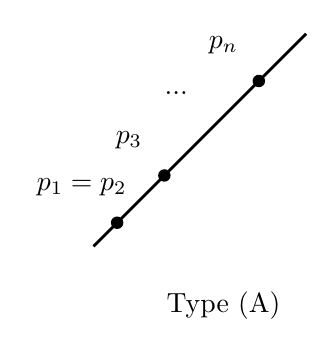
\begin{tikzpicture}[scale=3]
\draw[-,line width=1.0pt] (-0.5,-0.5) -- (0.4,0.4); 
\fill (-0.4,-0.4) circle (0.75pt);
\node at (-0.55,-0.25) {$p_1=p_2$};
\fill (-0.2,-0.2) circle (0.75pt);
\node at (-0.35,-0.05) {$p_3$};
\node at (-0.15,0.15) {$...$};
\node at (0.05,0.35) {$p_n$};
\fill (0.2,0.2) circle (0.75pt);
\node at (0.05, -0.75) {Type (A)};
\end{tikzpicture}
\mspace{70mu}
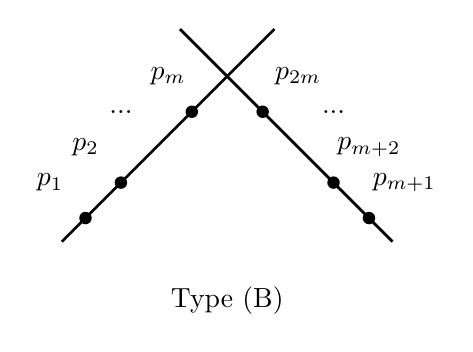
\begin{tikzpicture}[scale=3]
\draw[-,line width=1.0pt] (-0.5,-0.5) -- (0.4,0.4);
\draw[-,line width=1.0pt] (0.9,-0.5) -- (0,0.4);
\fill (-0.4,-0.4) circle (0.75pt);
\node at (-0.55,-0.25) {$p_1$};
\fill (-0.25,-0.25) circle (0.75pt);
\node at (-0.4,-0.1) {$p_2$};
\node at (-0.25,0.05) {$...$};
\node at (-0.05,0.2) {$p_m$};
\fill (0.05,0.05) circle (0.75pt);
\fill (0.8,-0.4) circle (0.75pt);
\node at (0.95,-0.25) {$p_{m+1}$};
\fill (0.65,-0.25) circle (0.75pt);
\node at (0.8,-0.1) {$p_{m+2}$};
\node at (0.65,0.05) {$...$};
\node at (0.5,0.2) {$p_{2m}$};
\fill (0.35,0.05) circle (0.75pt);
\node at (0.2,-0.75) {Type (B)};
\end{tikzpicture}
\end{equation*}
\end{center}

\noindent It is also clear that $\pi$ preserves the type (A) strata whilst contracting the type (B) ones to a (strictly semistable) point parametrizing the object
\begin{center}
\begin{equation*}
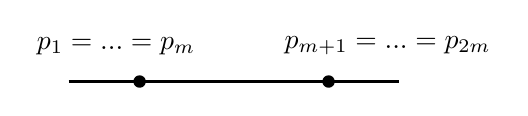
\begin{tikzpicture}[scale=3]
\draw[-,line width=1.0pt] (-0.5,0) -- (0.9,0);
\fill (0.6,0) circle (0.75pt);
\fill (-0.2,0) circle (0.75pt);
\node at (-0.3,0.15) {$p_1=...=p_m$};
\node at (0.85,0.15) {$p_{m+1}=...=p_{2m}$};
\end{tikzpicture}
\end{equation*}
\end{center}

\noindent The $\CC$-VHSs $\V^{\zeta_m^j}$ admit canonical extensions across the smooth part of $\overline{M}^H_{0,2m}\sm M_{0,2m}$, and we shall now compute the LMHS types there.

\begin{prop}\label{D5}
Along type \textup{(}A\textup{)} strata:
\begin{itemize}[leftmargin=0.5cm]
\item $\V_{\lim}^{\zeta_m^j}$ is pure of weight $1$, with $h^{1,0}=2m-2j-1$ and $h^{0,1}=2j-1$, unless $j=\tfrac{m}{2}$;
\item if $j=\tfrac{m}{2}$, then $h^{1,1}=h^{0,0}=1$, $h^{1,0}=h^{0,1}=m-1$, and $T=e^N$ \textup{(}with $N$ an isomorphism from the $(1,1)$ to $(0,0$ part\textup{)}; and
\item if $j>\tfrac{m}{2}$ \textup{[}resp.~$<\tfrac{m}{2}$\textup{]}, then we have the decomposition $\V^{\zeta_m^j}_{\lim}=\V_{\lim,1}^{\zeta_m^j}\oplus \V^{\zeta_m^j}_{\lim,\bar{\zeta}_m^{2j}}$ into $T=T_{\text{ss}}$-eigenspaces, where $\V^{\zeta_m^j}_{\lim,\bar{\zeta}_m^{2j}}$ is $1$-dimensional of type $(0,1)$ \textup{[}resp.~$(1,0)$\textup{]}.
\end{itemize}
\end{prop}
\begin{proof}
Begin by locally modeling (the effect on $C_{\ut}$ of) the collision of two points by $y^m+z^2=s$, as $s\to 0$. This has eigenspectrum
$$\textstyle\sum_{j=1}^{m-1}(\tfrac{3}{2}-\tfrac{j}{m},w(j),\tfrac{j}{m}),$$
where $w(j)=2$ if $j=\tfrac{m}{2}$ and $1$ otherwise.  Next, we apply the vanishing-cycle sequence (with $H^2_{\text{ph}}=\{0\}$ since the degenerate curve remains irreducible) to compute the LMHS. Finally, we perform a base-change by $s\mapsto s^2$ to preserve ordering of points, which squares the eigenvalues of the $T_{\text{ss}}$-action; in other words, we replace $\tfrac{3}{2}-\tfrac{j}{m}$ by $\{2(\tfrac{3}{2}-\tfrac{j}{m})\}+\lfloor \tfrac{3}{2}-\tfrac{j}{m}\rfloor$ ($\{\cdot\}$ denoting the fractional part), which gives the result.
\end{proof}

\begin{prop}\label{D6}
Along the type \textup{(}B\textup{)} strata, for each $1\leq j\leq m-1$, $\V^{\zeta_m^j}_{\lim}$ has Hodge numbers $h^{1,1}=h^{0,0}=1$, $h^{1,0}=2m-2j-2$, and $h^{0,1}=2j-2$; $N$ is an isomorphism from the $(1,1)$ to $(0,0)$ part, and $T=e^N$ is unipotent.
\end{prop}
\begin{proof}
In the GIT compactification for \emph{unordered} points, the degeneration is locally modeled by two copies of $y^m+x^m=s$, each with eigenspectrum
$$\textstyle\sum_{j=1}^{m-1}(1,2,\tfrac{j}{m})+\sum_{j=2}^{m-1}\sum_{k=1}^{j-1}(\tfrac{k+m-j}{m},1,\tfrac{j}{m})+\sum_{j=1}^{m-2}\sum_{k=j+1}^{m-1}(\tfrac{k+m-j}{m},1,\tfrac{j}{m}).$$
At this point one applies the vanishing-cycle sequence to deduce the form of the LMHS, noting that the degenerate curve is a union of $m$ $\PP^1$'s and $H^2_{\text{ph}}\cong \QQ(-1)^{\oplus m-1}$. For $\overline{M}^H_{0,2m}$, one then applies the base-change by $s\mapsto s^m$, which trivializes $T_{\text{ss}}$, allowing the extension class to vary along the type (B) stratum.
\end{proof}

\begin{example}
Combining \eqref{D1} with the two Propositions, $\V^{\bar{\zeta}_m}$ has Hodge-Deligne diagrams

\begin{align*}
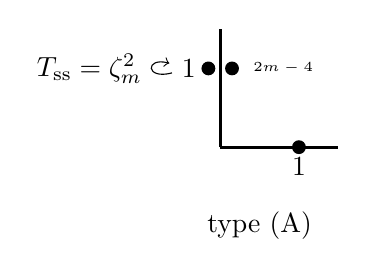
\begin{tikzpicture}[scale=0.5]
   	\node at (-0.8,2) (foo) {$1$};
    \path[->] (foo) edge  [loop left] node {$T_{\text{ss}}=\zeta_m^2$} ();
    \draw[-,line width=1.0pt] (0,0) -- (0,3);
    \draw[-,line width=1.0pt] (0,0) -- (3,0);
	\fill (2,0) circle (5pt);
	\node at (2,-0.5)  {$1$};		
	\fill (-0.3,2) circle (5pt);
	\fill (0.3,2) circle (5pt);	
	\node at (1.6,2) {\tiny$2m-4$};
	\node at (1,-2) {type (A)};	\end{tikzpicture}
& 
\begin{tikzpicture}[scale=0.5]
\draw[->,line width=1.0pt] (1.5,3.5) -- (0,3.5);
\node at (0.75,2.8) {$\lim$};
\node at (0,0) {\phantom{hh}};
\end{tikzpicture} 
&
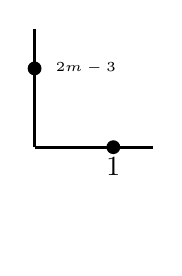
\begin{tikzpicture}[scale=0.5]
    \draw[-,line width=1.0pt] (0,0) -- (0,3);
    \draw[-,line width=1.0pt] (0,0) -- (3,0);
	\fill (2,0) circle (5pt);
	\fill (0,2) circle (5pt);		
	\node at (2,-0.5) {$1$};
	\node at (1.3,2) {\tiny$2m-3$};
	\node at (1,-2) {\phantom{$\V^{\bar{\zeta}_m}$}};				
\end{tikzpicture}
& 
\begin{tikzpicture}[scale=0.5]
\draw[->,line width=1.0pt] (0,3.5) -- (1.5,3.5);
\node at (0.75,2.8) {$\lim$};
\node at (0,0) {\phantom{hh}};
\end{tikzpicture} 
&
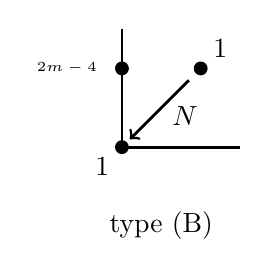
\begin{tikzpicture}[scale=0.5]
   	\node at (1.6,0.8) (foo) {$N$};
    \draw[-,line width=1.0pt] (0,0) -- (0,3);
    \draw[-,line width=1.0pt] (0,0) -- (3,0);
    \draw[->,line width=1.0pt] (1.7, 1.7) -- (0.2,0.2);
	\fill (0,2) circle (5pt);
	\fill (0,0) circle (5pt);	
	\node at (2.5,2.5) {$1$};	
	\fill (2,2) circle (5pt);
	\node at (-1.4,2) {\tiny$2m-4$};		\node at (-0.5,-0.5) {$1$};
	\node at (1,-2) {type (B)};
\end{tikzpicture}
\end{align*}


\noindent For $m=4$ resp.~$6$, the monodromy in type (A) is thus given by a complex reflection resp.~``triflection''.
\end{example}

\begin{rem}\label{D7}
For any $m$, $\V^{\bar{\zeta}_m}\,(\oplus \V^{\zeta_m})$ induces a map from the universal cover $\widetilde{M}_{0,2m}^{\text{un}}$ to a ball $\BB_{2m-3}$. Moreover, both LMHS types have $2m-4$ complex moduli. However, for $m$ different from $2,3,4,$ or $6$, this does not lead to a tidy extended period map: as the projection of the monodromy to $U(1,2m-3)$ is not discrete \cite{Mo}, the quotient of $\BB_{2m-3}$ by this is not Hausdorff. To circumvent this problem, we must replace $\BB_{2m-3}$ by its product with other (non-ball) symmetric domains, which receives the image of the period map for the $\QQ$-VHS $\oplus_{(j,m)=1}\V^{\zeta_m^j}$.
\end{rem}





%%%%%%%%%%%%%%%%%%%%%%%%%%%%%%%%%%%%%%
%%%%%%%%%%%%%%%%%%%%%%%%%%%%%%%%%%%%%%
\section{Hyperplane configurations and Dolgachev's conjecture}\label{S5}

Let $L_0,\ldots,L_{2n+1}\subset \PP^n$ be hyperplanes defined by linear forms $\ell_i$, in general position in the sense that $\cup L_i$ is a normal crossing divisor. Consider the $2{:}1$ cover $X\overset{\pi}{\twoheadrightarrow}\PP^n$ branched along $\cup L_i$, and the rank-$1$ $\QQ$-local system $\LL$ on $U=\PP^n\sm(\cup L_i)\overset{\jmath}{\hookrightarrow}\PP^n$ with monodromy $-1$ about each $L_i$. Since $X$ has finite quotient singularities, we have $\mathrm{IC}^{\bullet}_X=\QQ_X[n]$ and\footnote{See \cite[Prop.~8.2.30]{HTT} for the statement that $\mathrm{IC}^{\bullet}_{\PP^n}\LL=\jmath_*\LL[n]$.}
\begin{equation}\label{E1}
H:=H^n_{\pr}(X):=\frac{H^n(X)}{\pi^*H^n(\PP^n)}\cong H^n(\PP^n,\jmath_*\LL)\cong \IH^n(\PP^n,\LL)
\end{equation}
is a pure HS of weight $n$. By \cite[Lemma 8.2]{DK}, it has Hodge numbers
\begin{equation}\label{E2}
h^{p,n-p}_{\pr}(X)=\binom{n}{p}^2\;\;\implies\;\;h^n_{\pr}(X)=\binom{2n}{n}.	
\end{equation}
It is polarized by the intersection form $Q$, which presents no difficulties as $X$ has a smooth finite cover.

Taking $\cs\subset (\check{\PP}^n)^{2n+2}/\mathrm{PGL}_{n+1}(\CC)=:\csb$ to be the ($n^2$-dimensional) moduli space of $2n+2$ ordered hyperplanes in $\PP^n$ in general position, this construction yields a $\ZZ$-PVHS $\H\to \cs$ of CY-$n$ type with $H$ as reference fiber.  Let $\rho\colon \pi_1(\cs)\to \mathrm{Aut}(H,Q)^{\circ}=:M_{\max}$ be the monodromy representation of $\H$,\footnote{Here $(\cdot)^{\circ}$ means the identity component as algebraic group (i.e.~$\mathrm{SO}(H)$ instead of $O(H)$ if $n$ is even).} $\Pi$ its geometric monodromy group, and $M$ its Hodge (special Mumford-Tate) group. Here $\Pi$ is the identity connected component of $\widetilde{\Pi}:=\overline{\rho(\pi_1(\cs))}^{\QQ\text{-Zar}}$, and $\Pi\leq M\leq M_{\max}$. A conjecture attributed by \cite{SXZ} to Dolgachev states that the period map for $\H$ factors through a locally symmetric variety (also $n^2$-dimensional) of type $I_{n,n}$,\footnote{Note that the ``tautological VHS'' over $I_{n,n}$ is already geometrically realized by the $n^{\text{th}}$ primitive cohomology of a universal family of Weil abelian $2n$-folds.} which would imply that $\mathfrak{m}_{\RR}\cong \mathfrak{su}(n,n)$. This is equivalent to saying that,
\begin{equation}\label{E3}
\begin{split}
\text{\emph{up to finite data} (i.e.~after passing to a finite cover),}\phantom{hhh}	\\ \text{\emph{$\H$ is the $n^{\text{th}}$ wedge power of a VHS of weight $1$ and rank $2n$.}}
\end{split}
\end{equation}

The conjecture does hold for $n=1$ and $n=2$, but this merely reflects exceptional isomorphisms of Lie groups in low rank, namely $\mathrm{SU}(1,1)\cong \mathrm{SL}_2(\RR)$ and $\mathrm{SU}(2,2)\cong\mathrm{Spin}(2,4)^+$. That is, in both of these cases we \emph{also} have $\Pi\cong M_{\max}$ ($=\mathrm{SL}_2$ resp.~$\mathrm{SO}(2,4)$). For $n\geq 3$, in contrast, the conjecture would have $\Pi<M_{\max}$ a proper algebraic subgroup. In [op.~cit.] (and earlier works \cite{GSVZ,GSZ,GSZ2}), it was shown via quite computationally involved differential methods that in fact the monodromy is maximal for all $n$, and the conjecture fails for $n\geq 3$:

\begin{thm}\label{E4}
$\Pi=M=M_{\max}$ $\forall n\geq 1$.
\end{thm}

In the remainder of this section, we explain how asymptotic methods provide a much simpler approach to these results.  First we will give a careful argument disproving the conjecture for $n\geq 3$ odd, which \emph{a priori} is a weaker statement than the Theorem in that case. (The relation to the main theme of his paper --- specifically, to the setting of Cor.~\ref{A9} --- enters when we pass to the smooth finite cover $\hat{X}$ of $X$.) Then we sketch a proof of Theorem \ref{E4} using a more topological and monodromy-theoretic approach.

\subsection*{Disproof of \eqref{E3} for $n$ odd}

Most of the analysis that follows works for all $n$, though the last step is inconclusive for even $n$.

To begin, consider a pencil $\PP^1\overset{\ve}{\hookrightarrow}\csb$ of hyperplane configurations given by fixing $L_0,\ldots,L_{2n}$ (in general position) and letting $L_{2n+1}:=L_s$ vary along a line in $\check{\PP}^n$ (chosen to avoid linear spans of any $n-2$ $L_i$ in $\check{\PP}^n$).\footnote{It already follows from Zariski's theorem \cite[Thm.~3.22]{Vo} that $\rho(\pi_1(\PP^1\sm\Sigma))=\rho(\pi_1(\cs))$, but we won't need this.} Writing $\Sigma=\ve^{-1}(\csb\sm\cs)$, we have $|\Sigma|=\binom{2n+1}{n}$; and degenerations $\X_{\sigma}\to \Delta_{\sigma}$ of our double-covers at $\sigma\in \Sigma$ are locally modeled (with $t=s-\sigma$) by 
\begin{equation}\label{E5}
w^2\underset{\text{loc}}{=}x_1\cdots x_n(t-x_1-\cdots -x_n)	
\end{equation}
after a $\mathrm{PGL}_{n+1}(\CC)$-action. Accordingly, writing $X_0,\ldots,X_n$ for projective coordinates on $\PP^n$, we take $\ell_i=X_i$ for $0\leq i\leq n$ and $\ell_{2n+1}=tX_0-\sum_{i=1}^n X_i$, and $\ell_{n+1},\ldots,\ell_{2n}$ ``general''.

Let $\ul\colon \PP^n\hookrightarrow \PP^{2n+1}$ denote the linear embedding $[X_0{:}\cdots{:}X_n]\mapsto [\ell_0(\UX){:}\cdots {:}\ell_{2n+1}(\UX)]$, and $\phi\colon \PP^{2n+1}\to \PP^{2n+1}$ denote the map sending $[Z_0{:}\cdots {:}Z_{2n+1}]\mapsto [Z_0^2{:}\cdots {:}Z_{2n+1}^2]$. Then $\hat{X}:=\phi^{-1}(\ul(\PP^n))\subset \PP^{2n+1}$ is a smooth complete intersection on which\footnote{Here $\NP$ denotes the diagonal embedding.} $\A:=(\ZZ/2\ZZ)^{2n+2}/\NP(\ZZ/2\ZZ)$ acts via $\ue^{(i)}\mapsto \{Z_i\mapsto -Z_i\}$, with quotient $\PP^n$; explicitly, we have
\begin{equation}\label{E6}
\hat{X}=\textstyle\bigcap_{k=0}^n\{0=F_k(\UZ):=-Z_{n+k+1}^2+\ell_{n+k+1}(Z_0^2,\ldots,Z_n^2)\}.
\end{equation}
Write $\chi\in \mathrm{X}^*(\A)$ for the character sending each $\ue^{(i)}\mapsto -1$, $\A^{\circ}:=\ker(\chi)\leq \A$, and $q\colon \hat{X}\twoheadrightarrow X$ for the quotient by $\A^{\circ}$; then $H\cong q^* H^n_{\pr}(X)\cong H^n(\hat{X})^{\chi}$. Since $F_0(\UZ)=tZ_0^2-\sum_{i=1}^{n+1}Z_i^2$, we have thus replaced our original \emph{non}-isolated degeneration \eqref{E5} by a nodal one.

Next, we use the ``Cayley trick'' to replace the complete intersection $\hat{X}$ by a hypersurface
\begin{equation}\label{E7}
Y:=\{0=F:=\textstyle\sum_{k=0}^n Y_k F_k(\UZ)\}\subset \PP\left(\co_{\PP^{2n+1}}(2)^{\oplus n+1}\right)=:\mathbf{P}
\end{equation}
of dimension $3n$.  We have an $\A$-equivariant isomorphism $H^{3n}(Y)(n)\cong H^n(\hat{X})$ of HSs, so that $H\cong H^{3n}(Y)^{\chi}(n)$.  Notice that in affine coordinates $(z_1,\ldots,z_{2n+1};y_1,\ldots,y_n)$, $F=0$ becomes\footnote{Here ``h.o.t.'' means terms vanishing to order $3$ at the nodes.}
\begin{equation}\label{E8}
0=t-z_1^2-\cdots - z_{n+1}^2+\textstyle \sum_{k=1}^n y_k(b_k-z_{n+k+1})(b_k+z_{n+k+1})+\text{h.o.t},	
\end{equation}
where $b_k:=\sqrt{F_k(1,0,\ldots,0)}$. So at $t=0$, the singular fiber $Y_{\sigma}$ has $2^n$ nodes at $(Z_0;Z_1,\ldots,Z_{n+1};Z_{n+2},\ldots,Z_{2n+1};Y_0;Y_1,\ldots,Y_n)=$
\begin{equation}\label{E9}
\left(1;0,\ldots,0;(-1)^{a_1} b_1,\ldots,(-1)^{a_n}b_n;1;0,\ldots,0\right),\;\;\;\ua\in (\ZZ/2\ZZ)^n,	
\end{equation}
and the degeneration $\Y_{\sigma}\to \Delta_{\sigma}$ has smooth total space. The mixed spectrum of each node is $[(\tfrac{3n+1}{2},3n+1)]$ for $n$ odd and $[(\tfrac{3n+1}{2},3n)]$ for $n$ even; so $T_{\sigma}$ acts through multiplication by $(-1)^{n+1}$ on
\begin{equation}\label{E10}
H^{3n}_{\van}(Y_t)\cong \QQ(-\lfloor \tfrac{3n+1}{2} \rfloor)^{\oplus 2^n}.	
\end{equation}
Moreover, since the summands of \eqref{E10} are represented by $\eta_{\ua}=(-1)^{|\ua|}(dz_1\wedge \cdots \wedge dz_{2n+1}\wedge dy_1\wedge\cdots \wedge dy_n)/F^{\lceil\frac{3n+1}{2}\rceil}$ near the nodes \eqref{E9} (in the sense of \cite[\S2]{KL2}), it has a 1-dimensional subspace (generated by $\eta_{\chi}:=\sum (-1)^{|\ua|}\eta_{\ua}$) on which $\A$ acts through $\chi$.

Taking $\chi$-eigenspaces of the vanishing-cycle sequence for $\Y_{\sigma}\to \Delta_{\sigma}$ and twisting by $\QQ(n)$ now yields\small
\begin{equation}\label{E11}
0\to H^{3n}(Y_{\sigma})^{\chi}(n)\overset{\sp^{\chi}}{\to} \underset{\cong H_{\lim}}{\underbrace{H^{3n}_{\lim}(Y_t)^{\chi}(n)}}\overset{\can^{\chi}}{\to}\QQ(-\lfloor\tfrac{n+1}{2}\rfloor)\overset{\delta^{\chi}}{\to} H^{3n+1}_{\text{ph}}(Y_{\sigma})^{\chi}(n)\to 0	
\end{equation}\normalsize
We claim that $\delta=0$.  For $n$ even, this is clear, since $T_{\sigma}$ acts trivially on $H^{3n+1}_{\text{ph}}(Y_{\sigma})$ and by $-1$ on $\QQ(-\lfloor \tfrac{n+1}{2}\rfloor)$. So we conclude that $T_{\sigma}$ acts on $H_{\lim}$ via an orthogonal reflection. This doesn't factor through $\bigwedge^n$ of any automorphism of $\CC^{2n}$, but because it is finite (of order $2$), this does not (yet) disprove the conjecture.

On the other hand, for $n$ odd, it is not automatic that $\delta=0$. (This is a well-known problem with nodal degerenations in odd dimensions, cf.~\cite[\S2.2]{KL2}; and as we saw in the proof of Lemma \ref{E5}, our degenerations are finite quotients of nodal ones.) But if we can show $\delta=0$, then the conjecture is \emph{immediately} disproved (for odd $n\geq 3$).  Here is why: by \eqref{E6}, $H_{\lim}$ then has a class of type $(n+1,n+1)$, which must go to an $(n,n)$ class by $N_{\sigma}$,
\begin{center}
\begin{equation*}
	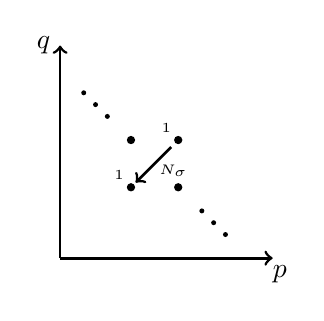
\begin{tikzpicture}[scale=0.3]
   	\node at (3.8,2.7) (foo) {\tiny$N_{\sigma}$};
    \draw[->,line width=1.0pt] (-1,-1) -- (-1,8);
    \draw[->,line width=1.0pt] (-1,-1) -- (8,-1);
    \draw[->,line width=1.0pt] (3.7, 3.7) -- (2.2,2.2);
	\fill (4,2) circle (5pt);
	\fill (2,4) circle (5pt);	
	\node at (1.5,2.5) {\tiny$1$};
	\fill (2,2) circle (5pt);
	\fill (4,4) circle (5pt);
	\node at (3.5,4.5) {\tiny$1$};
	\node at (8.3,-1.7) {$p$};
	\node at (-1.7,8) {$q$};
	\fill (1,5) circle (3pt);
	\fill (0.5,5.5) circle (3pt);
	\fill (0,6) circle (3pt);
	\fill (5,1) circle (3pt);
	\fill (5.5,0.5) circle (3pt);
	\fill (6,0) circle (3pt);
\end{tikzpicture}
\end{equation*}
\end{center}
forcing $\mathrm{rk}(N_{\sigma})=1$ (rather than $0$). (In different terms, each $T_{\sigma}$ is a nontrivial symplectic transvection.) But this is impossible for $\bigwedge^n$ of a nilpotent endomorphism of $\CC^{2n}$.

To complete the (dis)proof, then, we apply \cite[Thm.~2.9]{KL2}: for a nodal degeneration $Y\rightsquigarrow Y_{\sigma}$ of an odd-dimensional hypersurface of a smooth projective variety $\mathbf{P}$ satisfying Bott vanishing, the rank of $\delta$ is the number $m$ of nodes minus the rank of the map $$\mathrm{ev}\colon H^0(\mathbf{P},K_{\mathbf{P}}(\tfrac{3n+1}{2}Y_{\sigma}))\to \CC^m$$ given by evaluation at the nodes. The proof in [loc.~cit.] is equivariant in $\A$, and so we find that $\delta^{\chi}=0$ $\iff$ $\mathrm{ev}$ is nonzero on $H^0(\mathbf{P},K_{\mathbf{P}}(\tfrac{3n+1}{2}Y_{\sigma}))^{\chi}$, which can be checked at any node. Writing $\vec{\mathsf{e}}_1:=\sum_{i=0}^nY_i\tfrac{\d}{\d Y_i}$, $\vec{\mathsf{e}}_2:=\sum_{j=0}^{2n+1}Z_j\tfrac{\d}{\d Z_j}-2\vec{\mathsf{e}}_1$, and $\Omega:=\langle \vec{\mathsf{e}}_2,\langle \vec{\mathsf{e}}_1,d\UZ\wedge d\underline{Y}\rangle\rangle$, one checks that 
\begin{equation}\label{E12}
Y_0Z_0^2\Omega/(F_{t=0})^{\frac{3n+1}{2}}	
\end{equation}
is a well-defined section of $K_{\mathbf{P}}(\tfrac{3n+1}{2}Y_{\sigma})$ (cf.~\cite[\S4.5]{Ke}); and evidently $\A$ acts on it through $\chi$. Clearly, it is nonzero on the fiber of $K_{\mathbf{P}}(\tfrac{3n+1}{2}Y_{\sigma})$ at any of the nodes \eqref{E9}.


\subsection*{Sketch of proof of Theorem \ref{E4}}

Returning to the local picture \eqref{E5}, we now seek a more concrete topological description of the orthogonal reflections ($n$ even) and symplectic transvections ($n$ odd) through which $T_{\sigma}$ acts on $H$. So let $U_0\subset \mathbb{A}^n$ be the complement of the hyperplanes $x_1=0,\ldots,x_n=0$ and $x_1+\cdots +x_n=1$, and $\LL_0$ the rank-$1$ local system on $U_0$ with monodromies $-1$ about each of them. While the singularity $x_{\sigma}\overset{\imath_{\sigma}}{\hookrightarrow}X_{\sigma}$ ``at $\uo$'' in \eqref{E5} isn't isolated, the vanishing-cycle complex $\phi_t\QQ_{\X}$ is nothing but $\imath^{\sigma}_*V[-n]$, where $V:=\IH^n(\mathbb{A}^n,\LL_0)$ (as MHS). We begin with a local analogue of the covering argument just seen.

\begin{lem}\label{E13}
\textup{(i)} $\IH^n(\mathbb{A}^n,\LL_0)\cong \QQ(-\lfloor\tfrac{n+1}{2}\rfloor).$

\textup{(ii)} Local monodromy $T_{\sigma}$ acts on $V$ through multiplication by $(-1)^{n+1}$.

\textup{(iii)} The canonical map $\can_{\sigma}\colon H_{\lim}\to V$ is onto.
\end{lem}
\begin{proof}
Define maps 
\begin{itemize}[leftmargin=0.5cm]
\item $f_0\colon \mathbb{A}^n\hookrightarrow \mathbb{A}^{n+1}$ by $\ux\mapsto (\ux,1-\sum_{i=1}^n x_i)$, and
\item $\phi_0\colon \mathbb{A}^{n+1}\to\mathbb{A}^{n+1}$ by squaring all coordinates $z_i$;
\end{itemize}
then $\hat{X}_0:=\phi_0^{-1}(f_0(\mathbb{A}^n))\subset \mathbb{A}^{n+1}$ is the quadric hypersurface $\sum_{i=1}^{n+1}z_i^2=1$. The group $\A_0:=(\ZZ/2\ZZ)^{n+1}/\NP(\ZZ/2\ZZ)$ acts on $\hat{X}_0$ (multiplying coordinates by $\pm1$), with quotient $\mathbb{A}^n$. The quotient $q_0\colon \hat{X}_0\twoheadrightarrow X_0$ by the augmentation subgroup $\A_0^{\circ}$ yields the obvious $2{:}1$ branched cover of $\mathbb{A}^n$, with $H^n(X_0)\cong \IH^n(\mathbb{A}^n,\LL_0)$.

By the localization sequence for $\hat{X}_0$ (relative to its closure $\overline{\hat{X}}_0\subset \PP^{n+1}$) and weak Lefschetz, one easily shows that $H^j(\hat{X}_0)=0$ for $j\neq n$,\footnote{This simply recovers perversity of $\phi_f\QQ_{\X}[n]$.} and $H^n(\hat{X}_0)\cong \QQ(-\lfloor\tfrac{n+1}{2}\rfloor)$. (Writing $\d\hat{X}_0=\overline{\hat{X}}_0\sm\hat{X}_0$, this is $H^n(\overline{\hat{X}}_0)/H^{n-2}(\d\hat{X}_0)(-1)$ for $n$ even, and $\ker\{H^{n-1}(\d\hat{X}_0)(-1)\to H^{n+1}(\overline{\hat{X}}_0)\}$ for $n$ odd.) A generator for the \emph{dual} group $H^n_c(\hat{X}_0)$ is given by the real (vanishing) $n$-sphere $S^n_1:=\{\sum z_i^2=1\}\cap \RR^{n+1}$, whose class is invariant under $\A_0^{\circ}$ hence comes from $H^n_c(X_0)$. This gives (i).

The degeneration is modeled by replacing $\sum z_i^2=1$ by $\sum z_i^2=t$; as the spectrum of $\sum z_i^2$ is $[\tfrac{n+1}{2}]$, the monodromy is as described in (ii). Finally, (iii) follows from the last subsection since $\can_{\sigma}$ identifies with $\can^{\chi}$ in \eqref{E11}.
\end{proof}

The vanishing sphere $S^n_t:=\{\sum z_i^2=t\}\cap \RR^{n+1}$ in $\hat{X}_0$ has image in $X_0$ (by $q_0$) given by the double cover of $(\cap_{i=1}^n\{x_i\geq 0\})\cap \{\sum x_i\leq t\}$.  Let its image in $X$ (essentially via $\can^{\chi}\colon H^n_c(X_0)\to H^n(X)$) be denoted by $\nu_{\sigma}$; this is the vanishing cycle at $\sigma$, a ``double simplex'' branched along $\H_s$ and $n$ additional hyperplanes. It follows from (iii) that $T_{\sigma}$ is a transvection/reflection in $\nu_{\sigma}$. More precisely, rescaling $Q$ to have $Q(\nu_{\sigma},\nu_{\sigma})=\tfrac{1+(-1)^n}{2}$,
\begin{equation}\label{E14}
T_{\sigma}(u)=u-2Q(u,\nu_{\sigma})\nu_{\sigma}	
\end{equation}
for $u\in H$.

Now consider the general setting where $L_{2n+1}=L_s$, $L_0=\{X_0=0\}$, and the remaining $L_i$ are in general position. An easy extension of \eqref{E1} gives $H\cong \IH^n_c(\mathbb{A}^n,\LL)\cong H^n_c(X\sm L_0)$, whence $H^n_{\mathrm{pr}}(X)$ is spanned by double simplices branched along $n+1$ of the $L_{i\geq 0}$. Obviously all of these can be rewritten as $\ZZ$-linear combinations of double simplices branched along $L_s$ and $n$ of the $\{L_i\}_{1\leq i\leq 2n}$; call these $\nu_I$, where $I\subset \{1,\ldots,2n\}$ with $|I|=n$. Since $\mathrm{rk}H=\binom{2n}{n}$ and there are $\binom{2n}{n}$ of these vanishing cycles, they form a $\QQ$-basis of $H=H_{\text{pr}}^n(X)$. Write $T_I$ for the corresponding monodromies, and $\Gamma\leq \mathrm{Aut}(H_{\CC},Q)$ for the smallest $\CC$-algebraic group containing them; clearly $\Gamma\leq \widetilde{\Pi}_{\CC}$. Moreover, we note that if $|I\cap I'|=n-1$, then $Q(\nu_I,\nu_{I'})=\pm 1$ (rescaling as above, compatibly with \eqref{E14}).

Suppose then that $|I\cap I'|=n-1$.  If $n$ is odd, then $T_I(\nu_{I'})=\nu_I\pm \nu_{I'}=\pm T_{I'}^{-1}(\nu_I)$, whence $\nu_{I'}$ is in the $\Gamma$-orbit of $\nu_I$; so \emph{all} the $\nu_J$ are in the $\Gamma$-orbit of $\nu_I$. If $n$ is even, then reasoning as in \cite[\S4.4]{De},\footnote{See the paragraph after Lemme $4.4.3^{\text{s}}$.} $T_I T_{I'}^{\pm 1}$ is a transvection and its Zariski closure a $\mathbb{G}_a$ including transformations which send $\nu_I \mapsto \nu_{I'}$ and vice-versa; once again, all the $\nu_J$ are in the $\Gamma$-orbit of a single $\nu_I$.

Let $R:=\Gamma.\nu_I$ denote this orbit.  Obviously it spans $H_{\CC}$. Furthermore, for any $\delta\in R$, $\Gamma$ contains the transvection/reflection $T_{\delta}$: writing $\delta=\gamma.\nu_I$ ($\gamma\in \Gamma$), we have $T_{\delta}=T_{\gamma.\nu_I}=\gamma T_I\gamma^{-1}\in \Gamma$. So $\Gamma$ is in fact the $\CC$-algebraic closure of the $\{T_{\delta}\}_{\delta \in R}$, and we are exactly in the situation of \cite[Lemme 4.4.2]{De}. Conclude that $\Gamma=\mathrm{Aut}(H_{\CC},Q)$, hence $\widetilde{\Pi}=\mathrm{Aut}(H,Q)$, and thus $\Pi=\mathrm{Aut}(H,Q)^{\circ}$.

\begin{rem}\label{E15}
After writing this paper we encountered the article by \cite{Xu} which treats the more general setting of $r$-covers of $\PP^n$ branched along hyperplanes by considering local monodromies (as we have just done).  The argument is necessarily more complicated and technical than ours.  However, in the case $r=2$ (i.e., our setting) it appears to be incomplete.

If $r=2$ and $n$ is odd,  \cite[Prop.~3.4]{Xu} does not actually establish that $e_{(1)}$ (in the notation of [loc.~cit.]) is nonzero; this is exactly the issue regarding possible nonvanishing of $\delta$ dealt with above.  One could read \cite[Prop.~4.2]{Xu} as confirming this in retrospect, but this makes the argument quite convoluted.

If $r=2$ and $n$ is even, the proof of \cite[Prop.~4.2]{Xu} is wrong, as it makes use of the (false) statement that $\mathrm{Sp}_{2n}(\RR)$ ``does not admit any nontrivial one-dimensional invariant subspace'' in its action on $\bigwedge^n\RR^{2n}$.
\end{rem}



\begin{thebibliography}{?????}

\bibitem[Ar]{Ar} V. Arnol'd, \emph{Some problems in singularity theory}, Proc. Indian Acad. of Science 90 (1981), No. 1, 1-9.

\bibitem[Be]{Be} A. Beauville, \emph{Sur le nombre maximum de points doubles d'une surface dans $\PP^3$ $(\mu(5)=31)$}, Journe\'ees de G\'eometrie Alg\'ebrique d'Angers, Sijthoff \& Noordhoff, 1980, pp. 207-215.

\bibitem[Ca]{Ca} H. Cartan, \emph{Quotient d'une vari\'et\'e analytique par un groupe discret d'automorphismes}, S\'eminaire Henri Cartan 6 (1953-4), Expos\'e No.~12, 1-13.

\bibitem[Cs]{Cs} B. Castor, \emph{Bounding projective hypersurface singularities}, Washington University Ph.D. thesis, 2021.

\bibitem[De1]{De2} P. Deligne, \emph{Th\'eorie de Hodge II}, Publ. IHES 40 (1971), 5-57.

\bibitem[De2]{De} ---------, \emph{La conjecture de Weil II}, Publ. IHES 52 (1980), 137-252.

\bibitem[DM]{DM} P. Deligne and G. Mostow, \emph{Monodromy of hypergeometric functions and nonlattice integral monodromy}, Publ. IHES 63 (1986), 5-89.

\bibitem[Do]{Do} I. Dolgachev, \emph{Weighted projective varieties}, in ``Group actions and fields (Vancouver, B.C., 1981)'', 34-71, Lecture Notes in Math. 956, Springer, Berlin, 1982.

\bibitem[DK]{DK} I. Dolgachev and S. Kondo, \emph{Moduli of $K3$ surfaces and complex ball quotients}, in ``Arithmetic and geometry around hypergeometric functions'', 43-100, Progress in Math. 260, Birkh\"auser, Basel, 2007.

\bibitem[En]{En} S. Endra\ss, \emph{A projective surface of degree eight with 168 nodes}, J. Alg. Geom. 6 (1997), no. 2, 325-334.

\bibitem[GKS]{GKS} P. Gallardo, M. Kerr, and L. Schaffler, \emph{Geometric interpretation of toroidal compactifications of moduli of points in the line and cubic surfaces}, Adv. Math. 381 (2021), Paper No. 107632, 48 pp.

\bibitem[GSZ]{GSZ} R. Gerkmann, M. Sheng, and K. Zuo, \emph{Disproof of modularity of the moduli space of CY 3-folds of double covers of $\PP^3$ ramified along 8 planes in general position}, arXiv:0709.1051.


\bibitem[GSZ2]{GSZ2} ---------, \emph{Computational details of the disproof of modularity}, arXiv:0709.1054.

\bibitem[GSVZ]{GSVZ} R. Gerkmann, M. Sheng, D. van Straten, and K. Zuo, \emph{On the monodromy of the moduli space of Calabi-Yau threefolds coming from eight planes in $\PP^3$}, Math. Ann. 348 (2010), no. 1, 211-236.

\bibitem[Ha]{Ha} B. Hassett, \emph{Moduli spaces of weighted pointed stable curves}, Adv. Math. 173 (2003), no. 2, 316-352.

\bibitem[HTT]{HTT} R. Hotta, K. Takeuchi and T. Tanizaki, ``$D$-modules, perverse sheaves, and representation theory'' (trans. Takeuchi), Progress in Math. 236, Birkh\"auser Boston, Inc., Boston, 2008.

\bibitem[JR]{JR} D. Jaffe and D. Ruberman, \emph{A sextic surface cannot have 66 nodes}, J. Alg. Geom. 6 (1997), no. 1, 151-168.

\bibitem[Ke]{Ke} M. Kerr, ``Geometric construction of regulator currents with applications to algebraic cycles'', Princeton University Ph.D. thesis, 2003.

\bibitem[KL1]{KL1} M. Kerr and R. Laza, \emph{Hodge theory of degenerations, (I): consequences of the decomposition theorem}, with an appendix by M. Saito, Selecta Math. 27 (2021), no. 4, Paper No. 71, 48 pp.

\bibitem[KL2]{KL2} M. Kerr and R. Laza, \emph{Hodge theory of degenerations, (II): vanishing cohomology and geometric applications}, preprint, 2020, arXiv:2006.03953.

\bibitem[Mi]{Mi} Y. Miyaoka, \emph{The maximal number of quotient singularities on surfaces with given numerical invariants}, Math. Ann. 268 (1984), 159-171.

\bibitem[Mo]{Mo} G. Mostow, \emph{On discontinuous action of monodromy group on the complex $n$-ball}, J. Amer. Math. Soc. 1 (1988), no. 3, 555-586.

\bibitem[Sa]{Sa} M. Saito, \emph{Mixed Hodge modules}, Publ. Res. Inst. Math. Sci. 26 (1990), 221-333.

\bibitem[Sc]{Sc} C. Schoen, \emph{Algebraic cycles on certain desingularized nodal hypersurfaces}, Math. Ann. 270 (1985), no. 1, 17-27.

\bibitem[SXZ]{SXZ} M. Sheng, J. Xu and K. Zuo, \emph{The monodromy groups of Dolgachev's moduli spaces are Zariski dense}, Adv. Math. 272 (2015), 699-742.

\bibitem[St]{St} J. Steenbrink, \emph{Intersection form for quasi-homogeneous singularities}, Compos. Math. 34 (1977), no. 2, 211-223.

\bibitem[vS1]{vS1} D. van Straten, \emph{A quintic hypersurface in $\PP^4$ with 130 nodes}, Topology 32 (1993), no. 4, 857-864.

\bibitem[vS2]{vS2} ---------, \emph{The spectrum of hypersurface singularities}, arXiv:2003.00519.

\bibitem[Va]{Va} A. Varchenko, \emph{On the semicontinuity of the singularity spectrum and an upper bound for the number of singular points in projective hypersurfaces}, Doklady Ak. Nauk 270 (1983), no. 6, 1294-1297.

\bibitem[Vo]{Vo} C. Voisin, ``Hodge theory and complex algebraic geometry II'' (translated by L. Schneps), Cambridge Univ. Press, Cambridge, 2003.

\bibitem[Xu]{Xu} J. Xu, Zariski density of monodromy groups via Picard-Lefschetz type formula, IMRN 2018 (2018), 3556-3586.

\end{thebibliography}


\end{document}